\documentclass{oblivoir}
%%%Default packages
\usepackage{amsmath,amssymb,amsthm,kotex,tabu,graphicx,pifont}
\usepackage{../kswrapfig}

\usepackage{gensymb} %\degree

%%%More packages
%\usepackage{caption,subcaption}
%\usepackage[perpage]{footmisc}
%
\usepackage[skipabove=10pt,innertopmargin=10pt,nobreak=true]{mdframed}

\usepackage[inline]{enumitem}
\setlist[enumerate,1]{label=(\arabic*)}
\setlist[enumerate,2]{label=(\alph*)}

\usepackage{multicol}
\setlength{\columnsep}{30pt}
\setlength{\columnseprule}{1pt}
%
%\usepackage{forest}
%\usetikzlibrary{shapes.geometric,arrows.meta,calc}
%
%%%defi theo exam prob rema proo
%이 환경들 아래에 문단을 쓸 경우 살짝 들여쓰기가 되므로 \hspace{-.7em}가 필요할 수 있다.

\newcounter{num}
\newcommand{\defi}[1]
{\noindent\refstepcounter{num}\textbf{정의 \arabic{num})} #1\par\noindent}
\newcommand{\theo}[1]
{\noindent\refstepcounter{num}\textbf{정리 \arabic{num})} #1\par\noindent}
\newcommand{\revi}[1]
{\noindent\refstepcounter{num}\textbf{복습 \arabic{num})} #1\par\noindent}
\newcommand{\exam}[1]
{\bigskip\bigskip\noindent\refstepcounter{num}\textbf{예시 \arabic{num})} #1\par\noindent}
\newcommand{\prob}[1]
{\bigskip\bigskip\noindent\refstepcounter{num}\textbf{문제 \arabic{num})} #1\par\noindent}
\newcommand{\rema}[1]
{\bigskip\bigskip\noindent\refstepcounter{num}\textbf{참고 \arabic{num})} #1\par\noindent}
\newcommand{\proo}
{\bigskip\noindent\textsf{증명)}}

\newenvironment{talign}
 {\let\displaystyle\textstyle\align}
 {\endalign}
\newenvironment{talign*}
 {\let\displaystyle\textstyle\csname align*\endcsname}
 {\endalign}
%
%%%Commands

\newcommand{\procedure}[1]{\begin{mdframed}\vspace{#1\textheight}\end{mdframed}}

\newcommand\an[1]{\par\bigskip\noindent\textbf{문제 \ref{#1})}\par\noindent}

\newcommand\ann[2]{\par\bigskip\noindent\textbf{문제 \ref{#1})}\:\:#2\par\medskip\noindent}

\newcommand\ans[1]{\begin{flushright}\textbf{답 : }#1\end{flushright}}

\newcommand\anssec[1]{\bigskip\bigskip\noindent{\large\bfseries#1}}

\newcommand{\pb}[1]%\Phantom + fBox
{\fbox{\phantom{\ensuremath{#1}}}}

\newcommand\ba{\,|\,}

\newcommand\ovv[1]{\ensuremath{\overline{#1}}}
\newcommand\ov[2]{\ensuremath{\overline{#1#2}}}
%
%%%% Settings
%\let\oldsection\section
%
%\renewcommand\section{\clearpage\oldsection}
%
%\let\emph\textsf
%
%\renewcommand{\arraystretch}{1.5}
%
%%%% Footnotes
%\makeatletter
%\def\@fnsymbol#1{\ensuremath{\ifcase#1\or
%*\or **\or ***\or
%\star\or\star\star\or\star\star\star\or
%\dagger\or\dagger\dagger\or\dagger\dagger\dagger
%\else\@ctrerr\fi}}
%
%\renewcommand{\thefootnote}{\fnsymbol{footnote}}
%\makeatother
%
%\makeatletter
%\AtBeginEnvironment{mdframed}{%
%\def\@fnsymbol#1{\ensuremath{\ifcase#1\or
%*\or **\or ***\or
%\star\or\star\star\or\star\star\star\or
%\dagger\or\dagger\dagger\or\dagger\dagger\dagger
%\else\@ctrerr\fi}}%
%}   
%\renewcommand\thempfootnote{\fnsymbol{mpfootnote}}
%\makeatother
%
%%% 객관식 선지
\newcommand\one{\ding{172}}
\newcommand\two{\ding{173}}
\newcommand\three{\ding{174}}
\newcommand\four{\ding{175}}
\newcommand\five{\ding{176}}
\usepackage{tabto,pifont}
%\TabPositions{0.2\textwidth,0.4\textwidth,0.6\textwidth,0.8\textwidth}

\newcommand\taba[5]{\par\noindent
\one\:{#1}
\tabto{0.2\textwidth}\two\:\:{#2}
\tabto{0.4\textwidth}\three\:\:{#3}
\tabto{0.6\textwidth}\four\:\:{#4}
\tabto{0.8\textwidth}\five\:\:{#5}}

\newcommand\tabb[5]{\par\noindent
\one\:{#1}
\tabto{0.33\textwidth}\two\:\:{#2}
\tabto{0.67\textwidth}\three\:\:{#3}\medskip\par\noindent
\four\:\:{#4}
\tabto{0.33\textwidth}\five\:\:{#5}}

\newcommand\tabc[5]{\par\noindent
\one\:{#1}
\tabto{0.5\textwidth}\two\:\:{#2}\medskip\par\noindent
\three\:\:{#3}
\tabto{0.5\textwidth}\four\:\:{#4}\medskip\par\noindent
\five\:\:{#5}}

\newcommand\tabd[5]{\par\noindent
\one\:{#1}\medskip\par\noindent
\two\:\:{#2}\medskip\par\noindent
\three\:\:{#3}\medskip\par\noindent
\four\:\:{#4}\medskip\par\noindent
\five\:\:{#5}}
%
%%%% fonts
%
%\usepackage{fontspec, xunicode, xltxtra}
%\setmainfont[]{은 바탕}
%\setsansfont[]{은 돋움}
%\setmonofont[]{은 바탕}
%\XeTeXlinebreaklocale "ko"
%%%%
\begin{document}

\title{수학(하) : 11 유리함수와 무리함수의 그래프}
\author{}
\date{\today}
\maketitle
\tableofcontents
\newpage

%%프
\section{복습}
\begin{mdframed}
%
\theo{도형의 평행이동}\label{review1}
도형 \(f(x,y)=0\)을 \(x\)축의 방향으로 \(a\)만큼, \(y\)축의 방향으로 \(b\)만큼 평행이동시키면 \(f(x-a,\: y-b)=0\)이 된다.
\[f(x,y)=0
\quad\xrightarrow[x\:\leftarrow\: x-a,\quad y\:\leftarrow\: y-b\:\:대입]
{\fbox{$x$}\::\:a,\quad\fbox{$y$}\::\:b}\quad
f(x-a,\: y-b)=0\]
\end{mdframed}

%
\exam{}\label{review2}
포물선 \(y=x^2\)를 \(x\)축의 방향으로 \(2\)만큼, \(y\)축의 방향으로 \(3\)만큼 평행이동시키면 \(y-3=(x-2)^2\)이 된다.
\[y=x^2
\quad\xrightarrow[x\:\leftarrow\: x-2,\quad y\:\leftarrow\: y-3\:\:대입]
{\fbox{$x$}\::\:2,\quad\fbox{$y$}\::\:3}\quad
y-3=(x-2)^2\]
이것을 정리하면 \(y=(x-2)^2+3\)이 된다.
\begin{center}
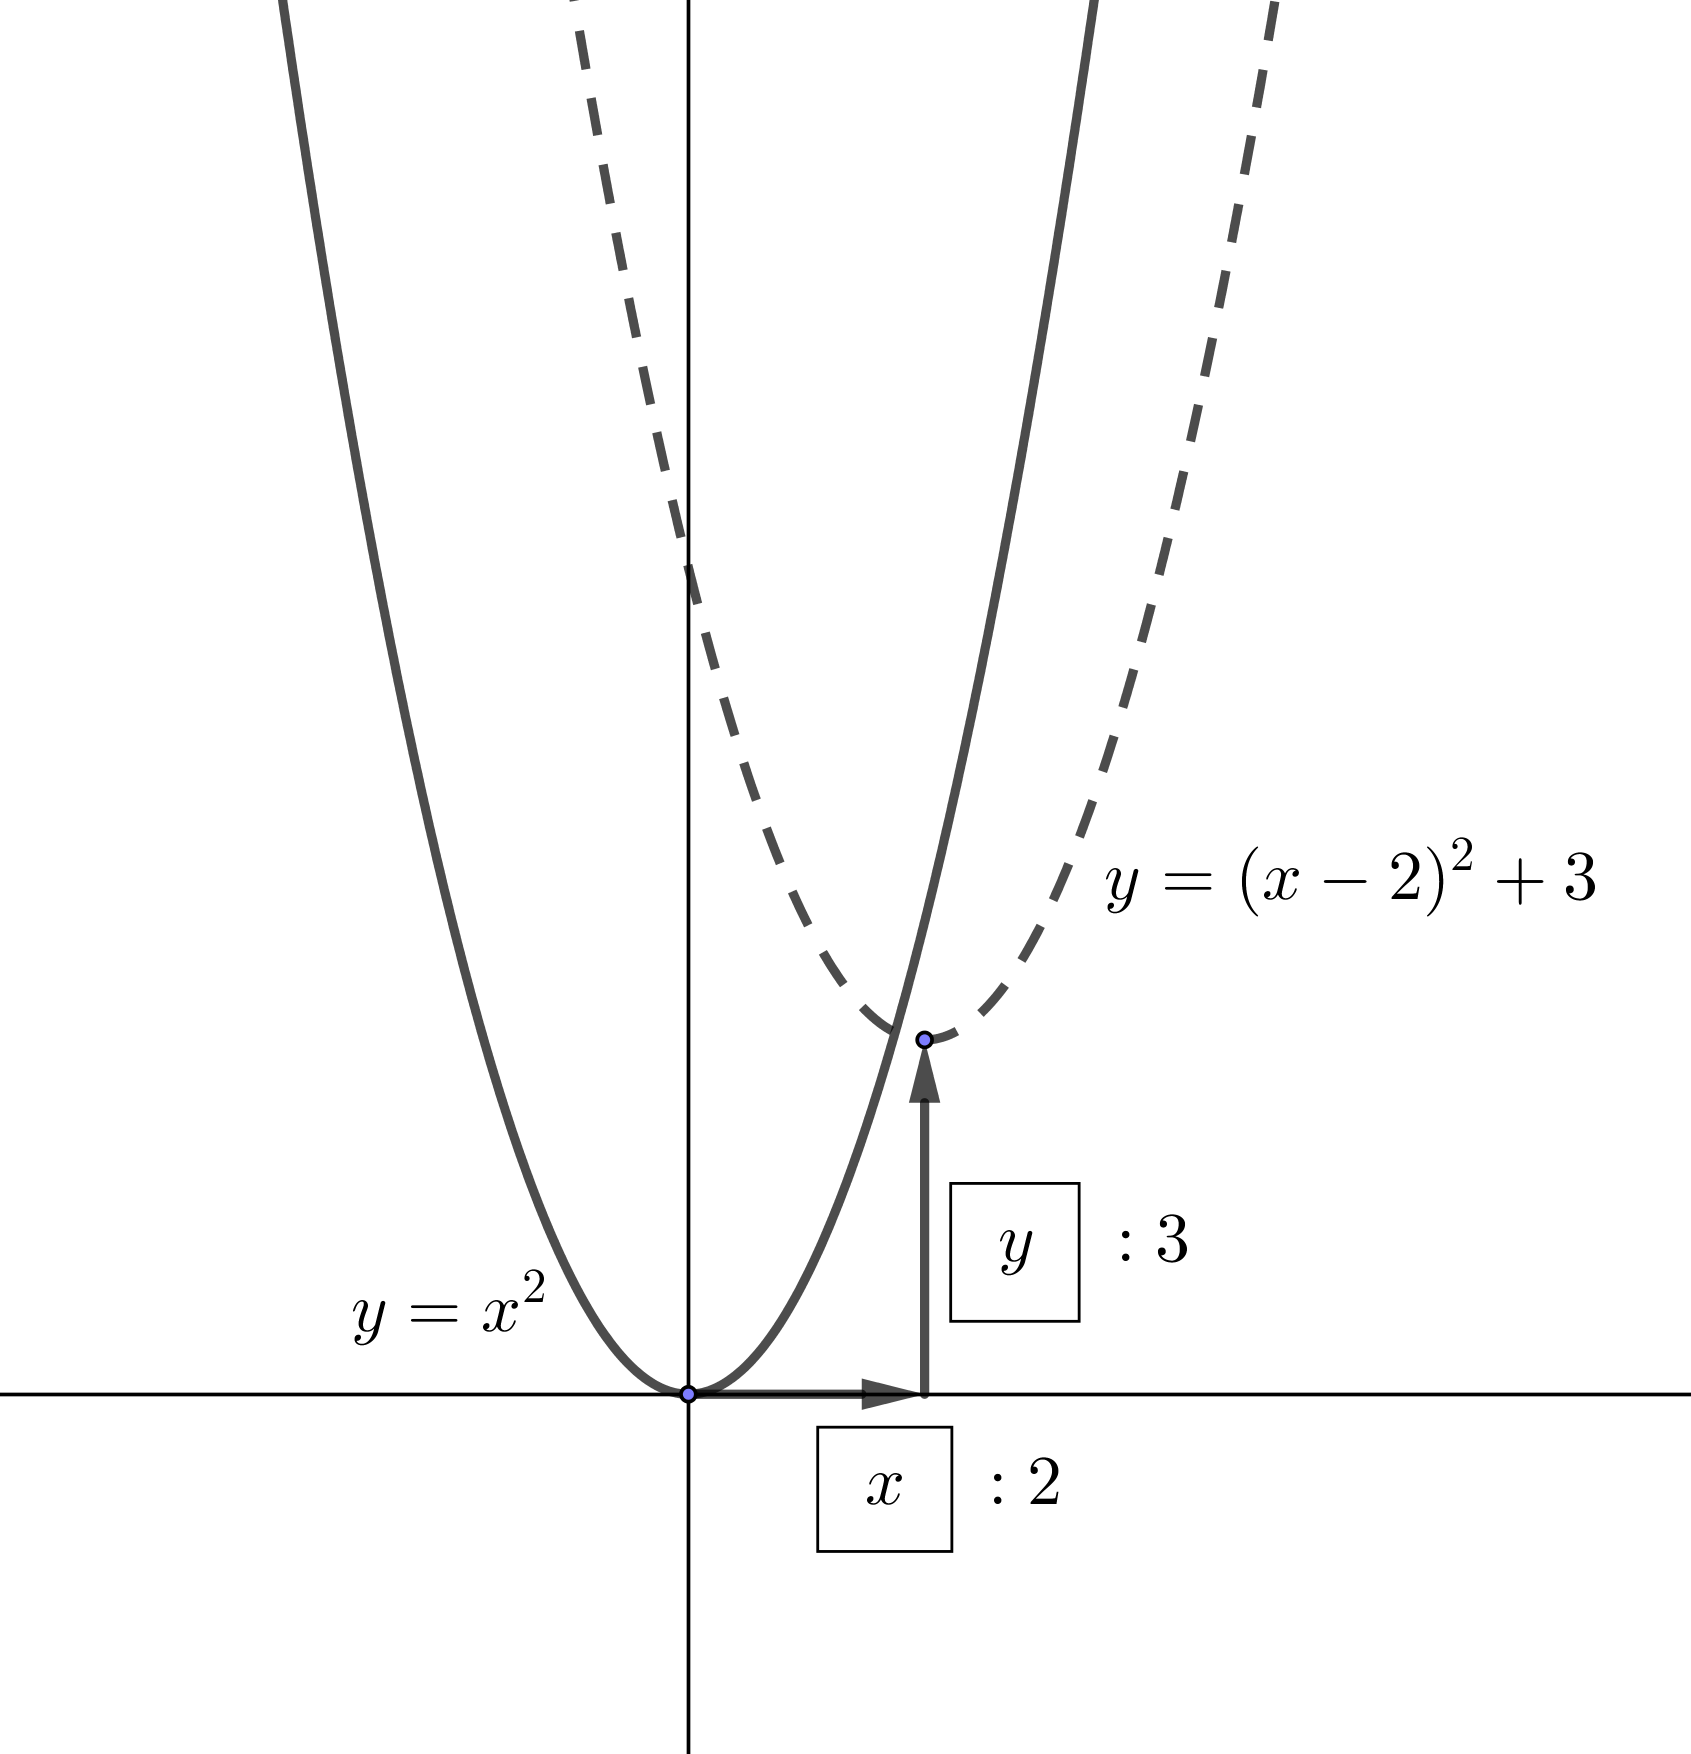
\includegraphics[width=0.5\textwidth]{review_2}
\end{center}

%
\prob{}\label{review3}
직선 \(y=3x\)을 \(x\)축의 방향으로 \(1\)만큼, \(y\)축의 방향으로 \(-2\)만큼 평행이동시킨 도형의 방정식을 구하여라.

\begin{mdframed}
%
\theo{도형의 대칭이동}\label{rreflect3}
도형 \(f(x,y)=0\)을 각각 \(x\)축, \(y\)축, 원점,  \(y=x\)에 대해 대칭이동시키면
\begin{gather*}
f(x,y)=0
\quad\xrightarrow[y\:\leftarrow\: -y\:\:대입]{x축\:\:대칭}\quad
f(x,-y)=0
\\[10pt]
f(x,y)=0
\quad\xrightarrow[x\:\leftarrow\: -x\:\:대입]{y축\:\:대칭}\quad
f(-x,y)=0
\\[10pt]
f(x,y)=0
\quad\xrightarrow[x\:\leftarrow\: -x,\quad y\:\leftarrow\: -y\:\:대입]{원점\:\:대칭}\quad
f(-x,-y)=0
\\[10pt]
f(x,y)=0
\quad\xrightarrow[x\:\leftarrow\: y,\quad y\:\leftarrow\: x\:\:대입]{y=x\:\:대칭}\quad
f(y,x)=0
\end{gather*}
\end{mdframed}

%
\exam{원 \((x-3)^2+(y-1)^2=1\)을}\\[-5pt]\label{review5}
\begin{enumerate*}[itemjoin=\tabto{.5\textwidth}]
\item
\(x\)축에 대해
\item
\(y\)축에 대해
\end{enumerate*}\par\bigskip\noindent
대칭이동시킨 도형의 방정식을 구하여라.
\begin{mdframed}
\[(1)\:\:
(x-3)^2+(y-1)^2=1
\quad\xrightarrow[y\:\leftarrow\: -y\:\:대입]{x축\:\:대칭}\quad
(x-3)^2+(-y-1)^2=1\]
이다.
이것을 정리하면
\((x-3)^2+(y+1)^2=1\)이 된다.

\[(2)\:\:
(x-3)^2+(y-1)^2=1
\quad\xrightarrow[x\:\leftarrow\: -x\:\:대입]{y축\:\:대칭}\quad
(-x-3)^2+(y-1)^2=1\]
이다.
이것을 정리하면
\((x+3)^2+(y-1)^2=1\)이 된다.
\end{mdframed}

%
\prob{예시 \ref{review5})의 도형을}\\[-5pt]\label{review6}
\begin{enumerate*}[itemjoin=\tabto{.5\textwidth}]
\item
원점 대해
\item
직선 \(y=x\)에 대해
\end{enumerate*}\par\bigskip\noindent
대칭이동시킨 도형의 방정식을 구하여라.


%\begin{mdframed}
%%
%\theo{역함수와 그 그래프}\label{review4}
%%함수 \(y=f(x)\)의 역함수 \(y=f^{-1}(x)\)를 구할 때에는 \(y=f(x)\)의 식에 \(x\) 대신에 \(y\)를, \(y\) 대신에 \(x\)를 대입하여 정리하면 얻어진다.
%%따라서 \(y=f(x)\)의 그래프와 \(y=f^{-1}(x)\)의 그래프는 직선 \(y=x\)에 대하여 대칭이다.
%일대일대응인 함수 \(f\)에 대하여,\\
%\(y=f(x)\)의 그래프와 \(y=f^{-1}(x)\)의 그래프는 직선 \(y=x\)에 대하여 대칭이다.
%\[y=f(x)
%\quad\xrightarrow[x\:\leftarrow\:y,\quad y\:\leftarrow\:x\:\:대입]
%{y=x\:\:대칭}\quad
%y=f^{-1}(x)\]
%\end{mdframed}
%
%\exam{}\label{review5}
%함수 \(y=2x\)에서 \(x\) 대신 \(y\)를, \(y\) 대신 \(x\)를 대입하면 \(x=2y\)이다.
%이것을 정리하면 \(y=-\frac12x\)가 된다.
%\[y=-2x
%\quad\xrightarrow[x\:\leftarrow\:y,\quad y\:\leftarrow\:x\:\:대입]
%{y=x\:\:대칭}\quad
%y=-\frac12x\]
%\begin{center}
%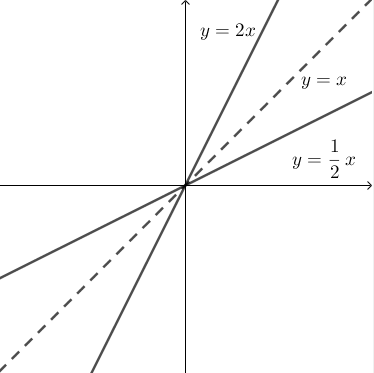
\includegraphics[width=0.5\textwidth]{review_5}
%\end{center}
%
%%
%\prob{}\label{review6}
%함수 \(y=\frac13x+1\)의 역함수를 구하여라.

%%
\section{유리함수의 그래프}
%
\exam{\(y=\frac1x\)의 그래프를 그려라.}
\begin{mdframed}\label{rational1}
\(y=\frac1x\)를 만족시키는 모든 점 \((x,y)\)을 표시하면 된다.\\
\(x=1\)이면 \(y=1\)이고 \(y=2\)이면 \(y=\frac12\)이다.
따라서 \(y=\frac1x\)의 그래프는 \((1,1)\), \((2,\frac12)\)와 같은 점들을 포함한다.
이밖에도
\begin{align*}
(x,y)
=&\textstyle(1,1),\:(2,\frac12),\:(3,\frac13),\:(4,\frac14),\:\cdots\\
&\textstyle(\frac12,2),\:(\frac13,3),\:(\frac14,4),\:\cdots\\
&\textstyle(-1,-1),\:(-2,-\frac12),\:(-3,-\frac13),\:(-4,-\frac14),\:\cdots\\
&\textstyle(-\frac12,-2),\:(-\frac13,-3),\:(-\frac14,-4),\:\cdots
\end{align*}
와 같은 점들을 찍을 수 있다.
이 점들을 자연스럽게 이으면 다음과 같은 곡선이 나온다.
\begin{center}
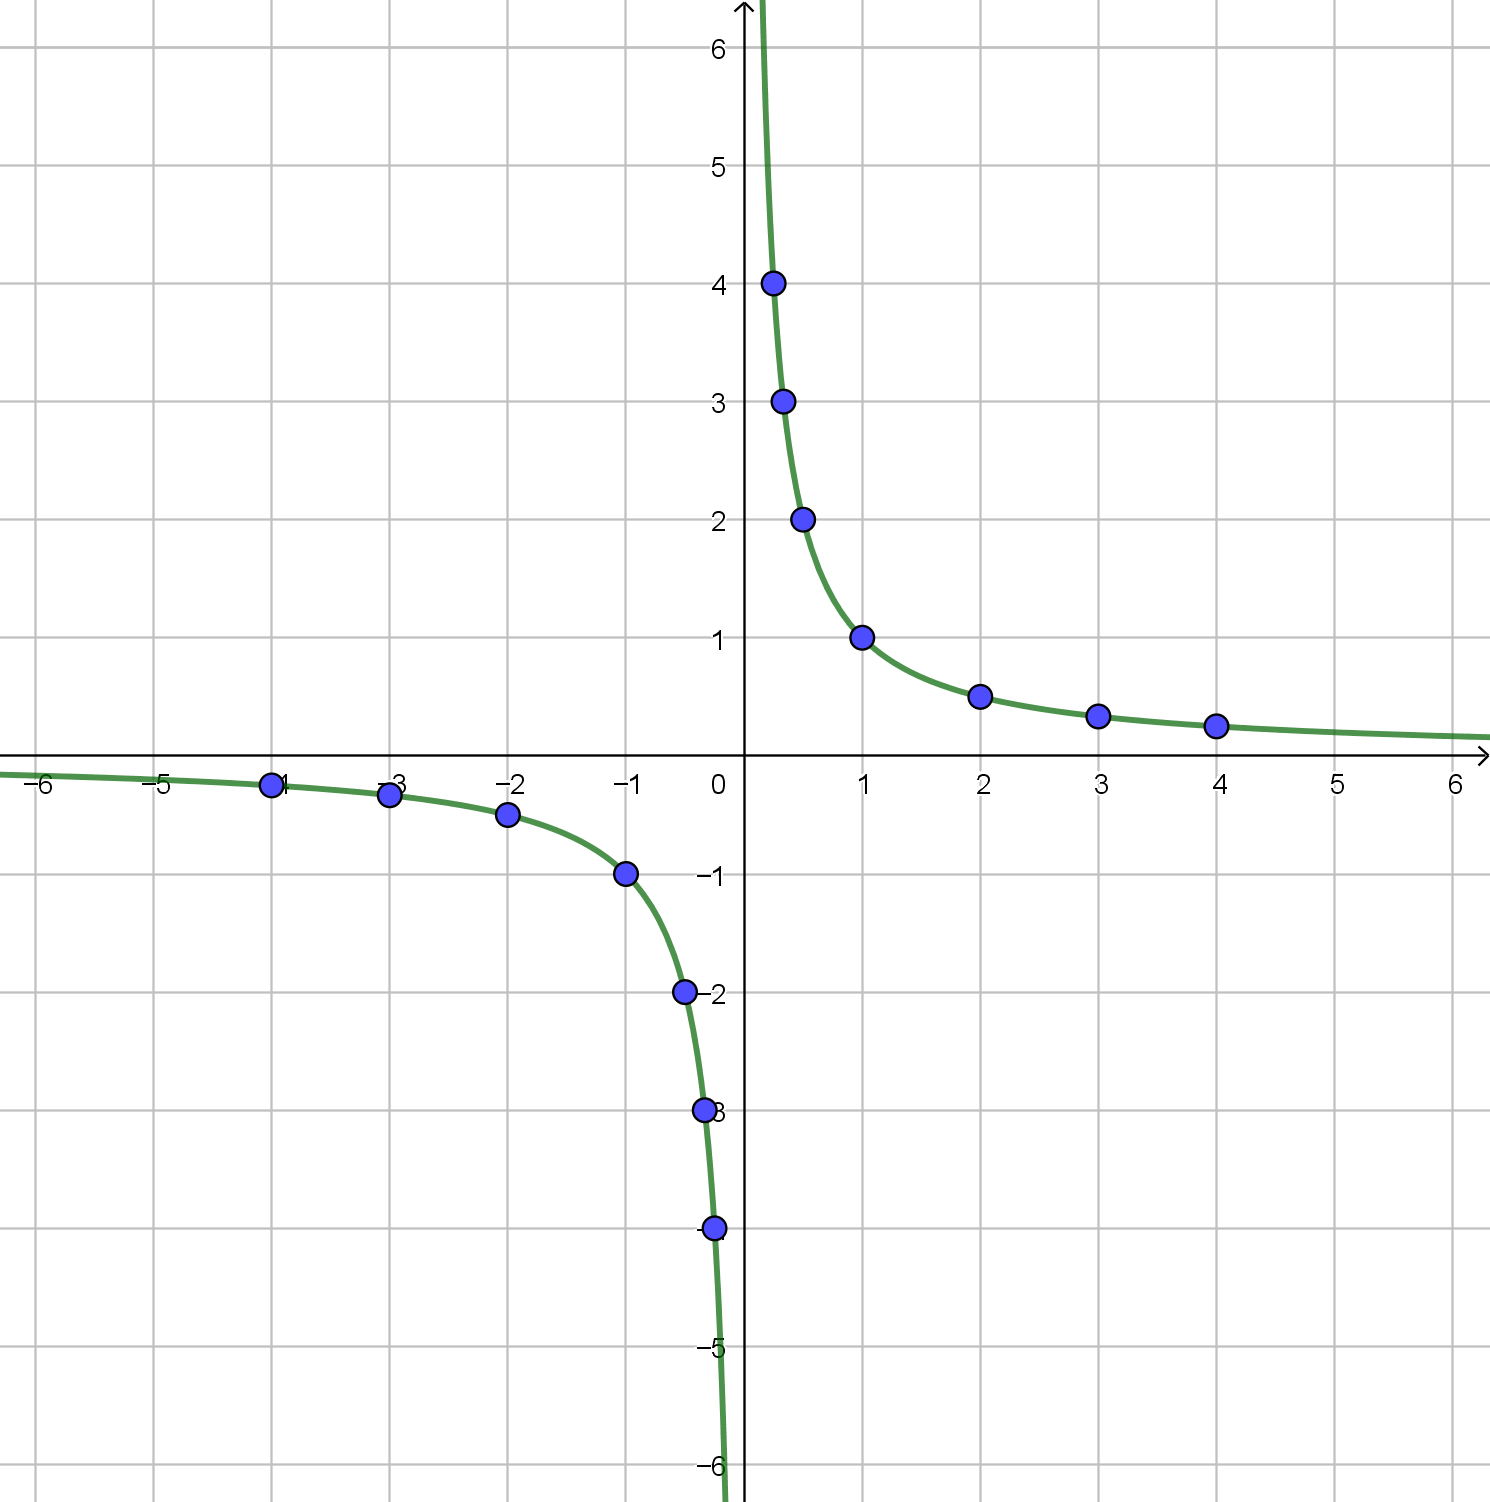
\includegraphics[width=0.85\textwidth]{rational_1}
\end{center}
\end{mdframed}

%
\prob{다음 유리함수들의 그래프를 그려라.}
\begin{enumerate}\label{rational2}
\item
\(y=\frac2x\)
\item
\(y=\frac6x\)
\item
\(y=\frac1{2x}\)
\end{enumerate}
\begin{center}
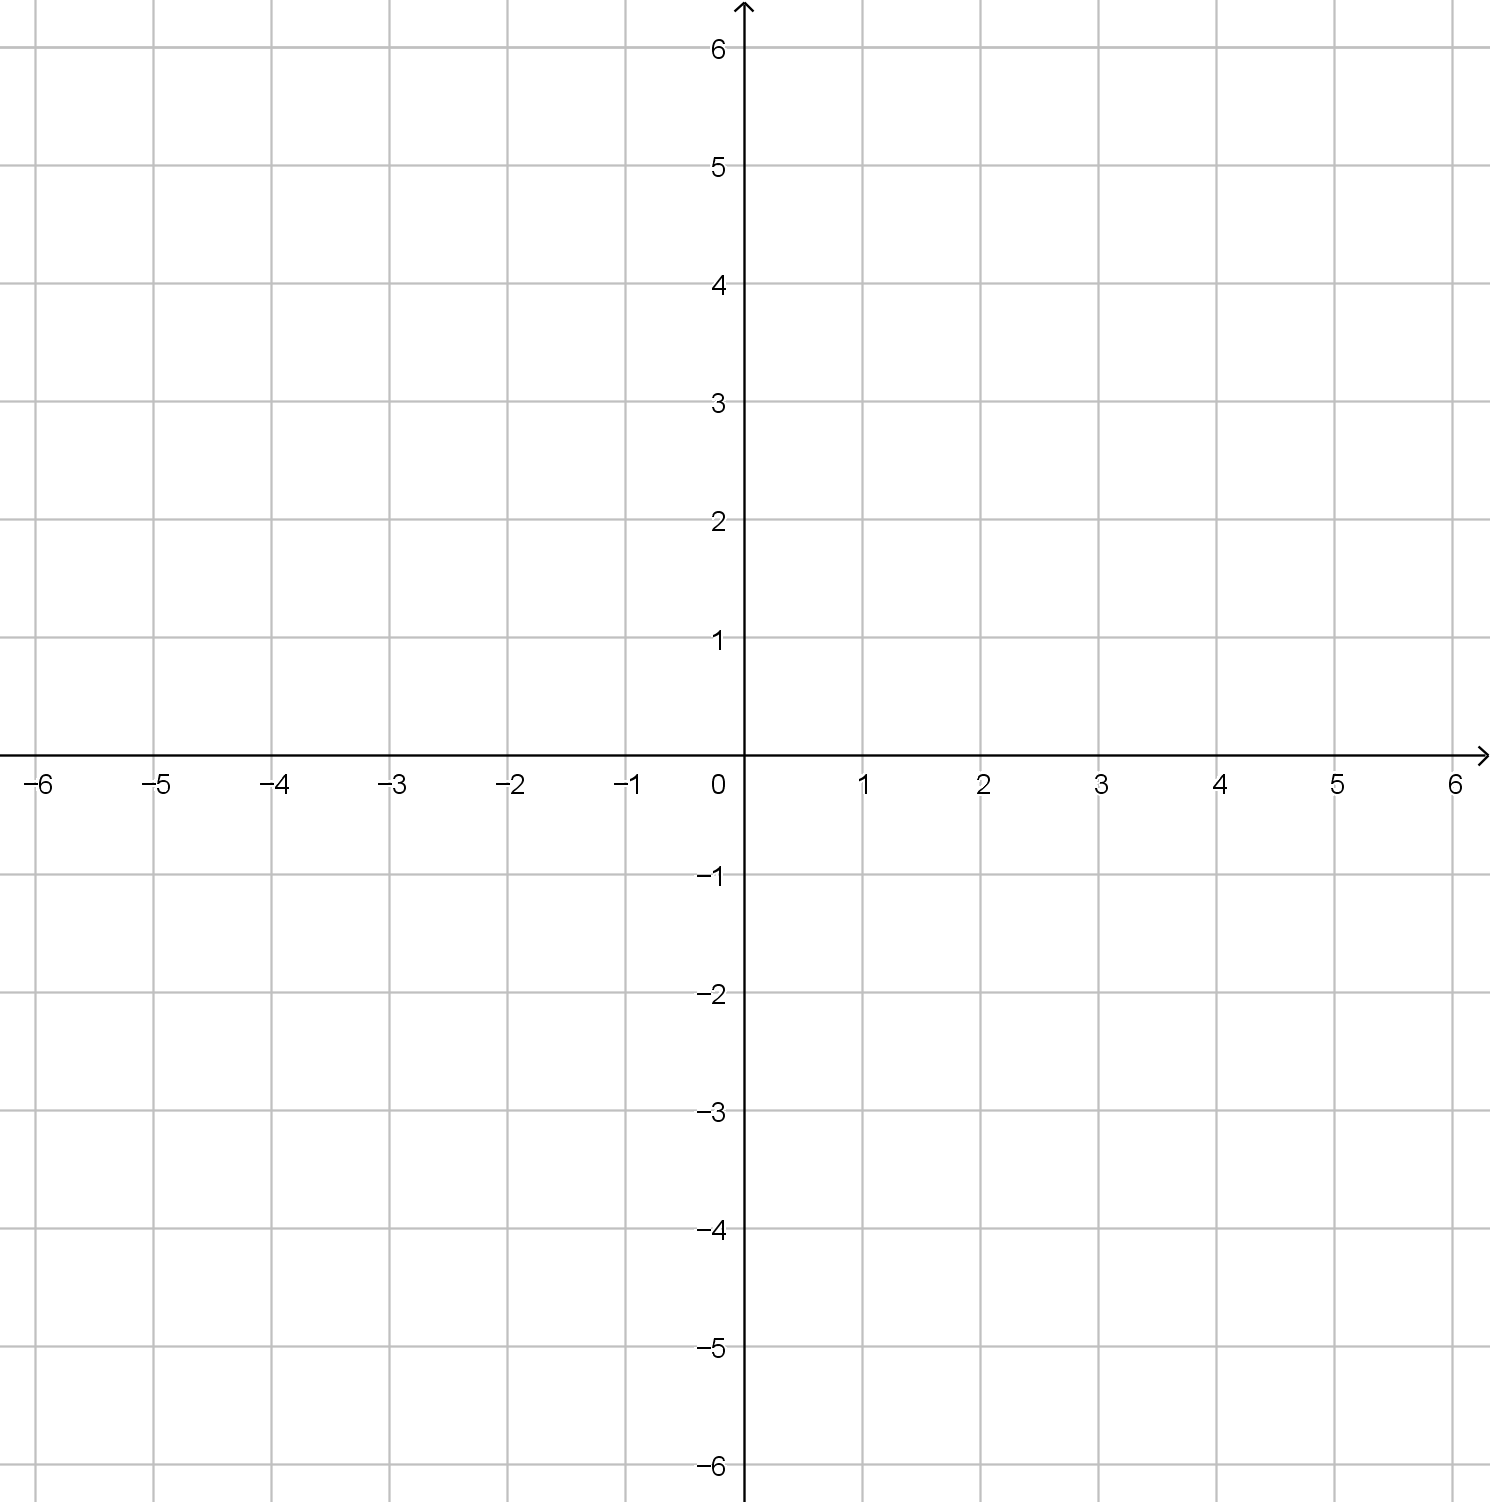
\includegraphics[width=0.8\textwidth]{66grid}
\end{center}

\begin{mdframed}
%
\theo{\(y=\frac kx\)의 그래프(\(k>0\))}
\begin{itemize}\label{rational3}
\item
대칭적인 곡선이다.\footnotemark
\item
제1사분면과 제3사분면에 그래프가 그려진다.
\item
\(k\)값이 커질수록 원점에서 멀어지고 \(k\)값이 작아질수록 원점에 가까워진다.
\end{itemize}
\end{mdframed}
\footnotetext{원점에 대해, 직선 \(y=x\)에 대해, 직선 \(y=-x\)에 대해 대칭인 곡선이다.}

%
\exam{\(y=-\frac1x\)의 그래프를 그려라.}
\begin{mdframed}\label{rational4}
마찬가지로
\(y=-\frac1x\)를 만족시키는 모든 점 \((x,y)\)을 표시하면 된다.\\
\begin{align*}
(x,y)
=&\textstyle(1,-1),\:(2,-\frac12),\:(3,-\frac13),\:(4,-\frac14),\:\cdots\\
&\textstyle(\frac12,-2),\:(\frac13,-3),\:(\frac14,-4),\:\cdots\\
&\textstyle(-1,1),\:(-2,\frac12),\:(-3,\frac13),\:(-4,\frac14),\:\cdots\\
&\textstyle(-\frac12,2),\:(-\frac13,3),\:(-\frac14,4),\:\cdots
\end{align*}
와 같은 점들을 찍을 수 있다.
이번에도 이 점들을 자연스럽게 이으면 다음과 같은 곡선이 나온다.
\begin{center}
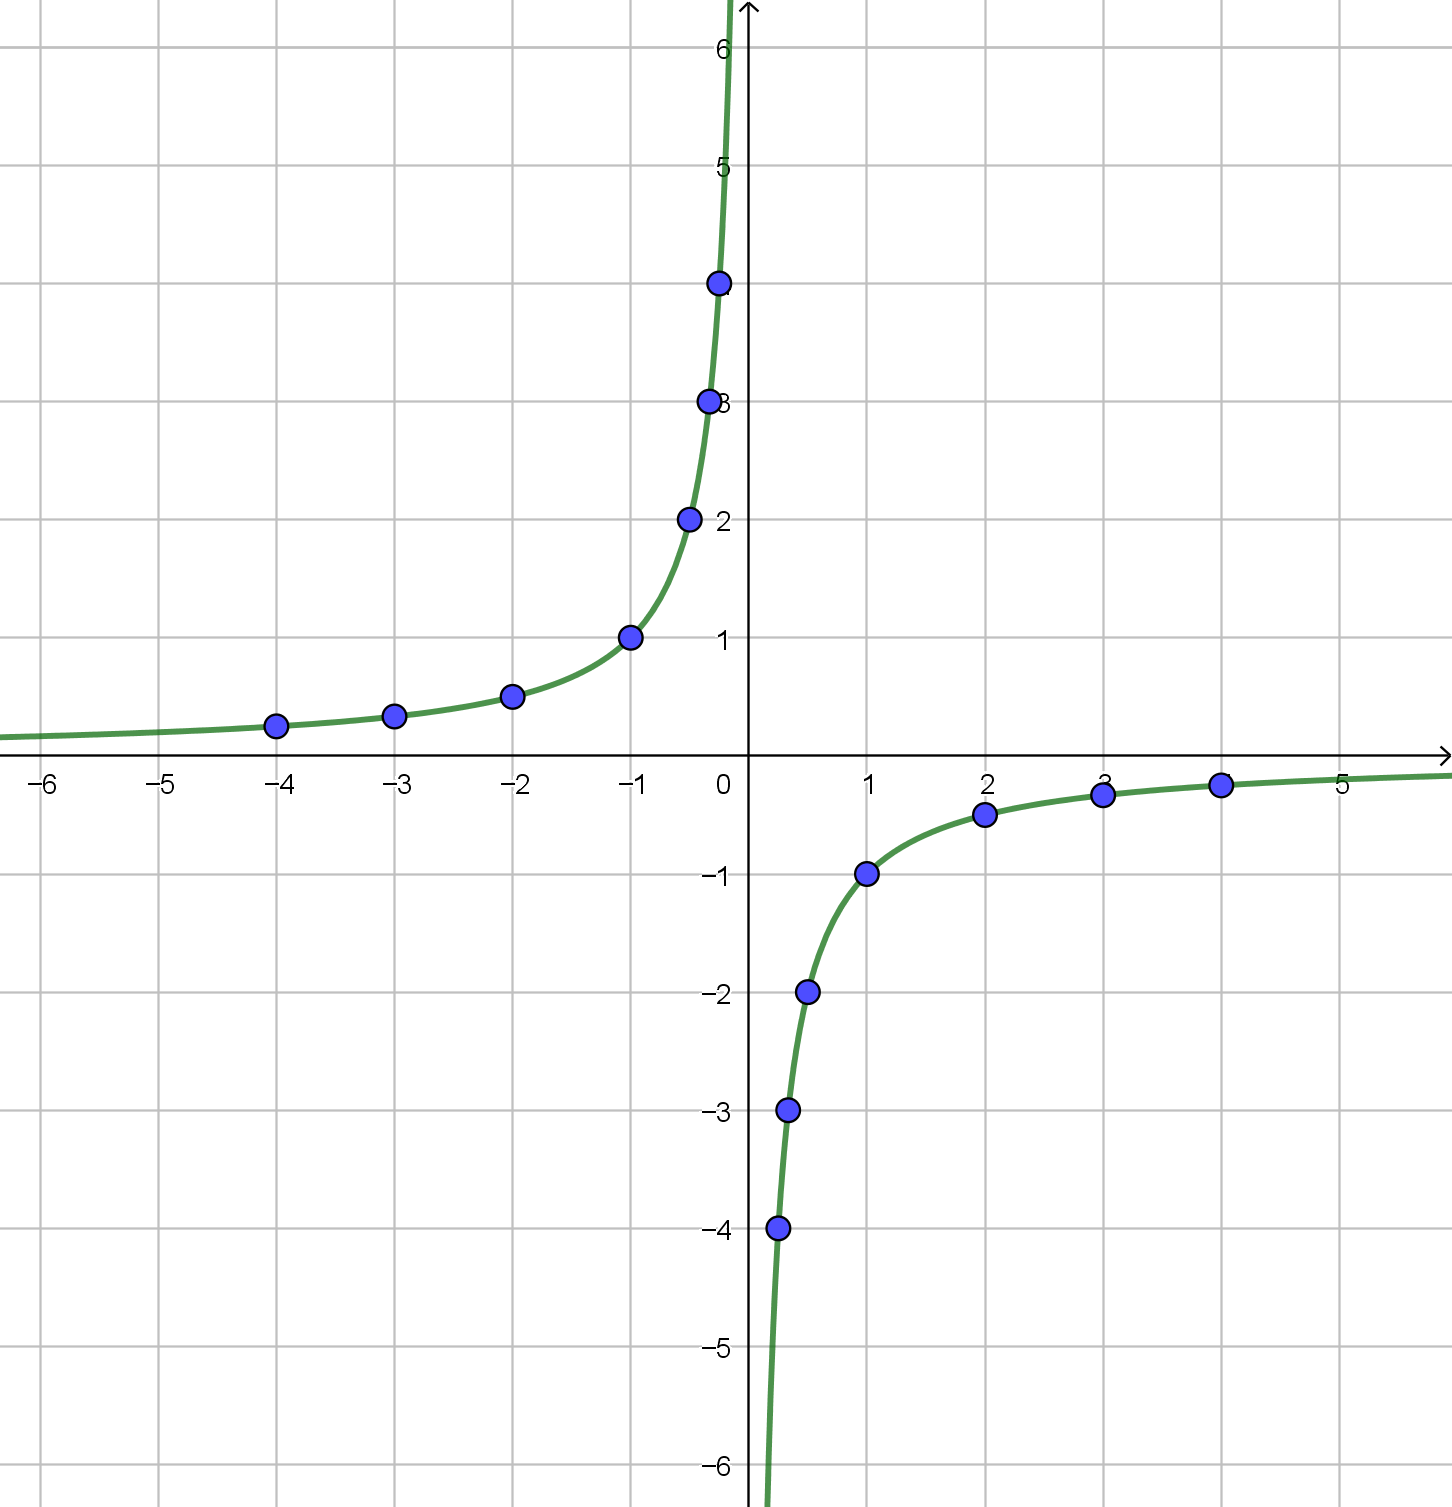
\includegraphics[width=0.85\textwidth]{rational_4}
\end{center}
\end{mdframed}

\newpage
%
\prob{다음 유리함수들의 그래프를 그려라.}
\begin{enumerate}\label{rational5}
\item
\(y=-\frac2x\)
\item
\(y=-\frac6x\)
\item
\(y=-\frac1{2x}\)
\end{enumerate}
\begin{center}
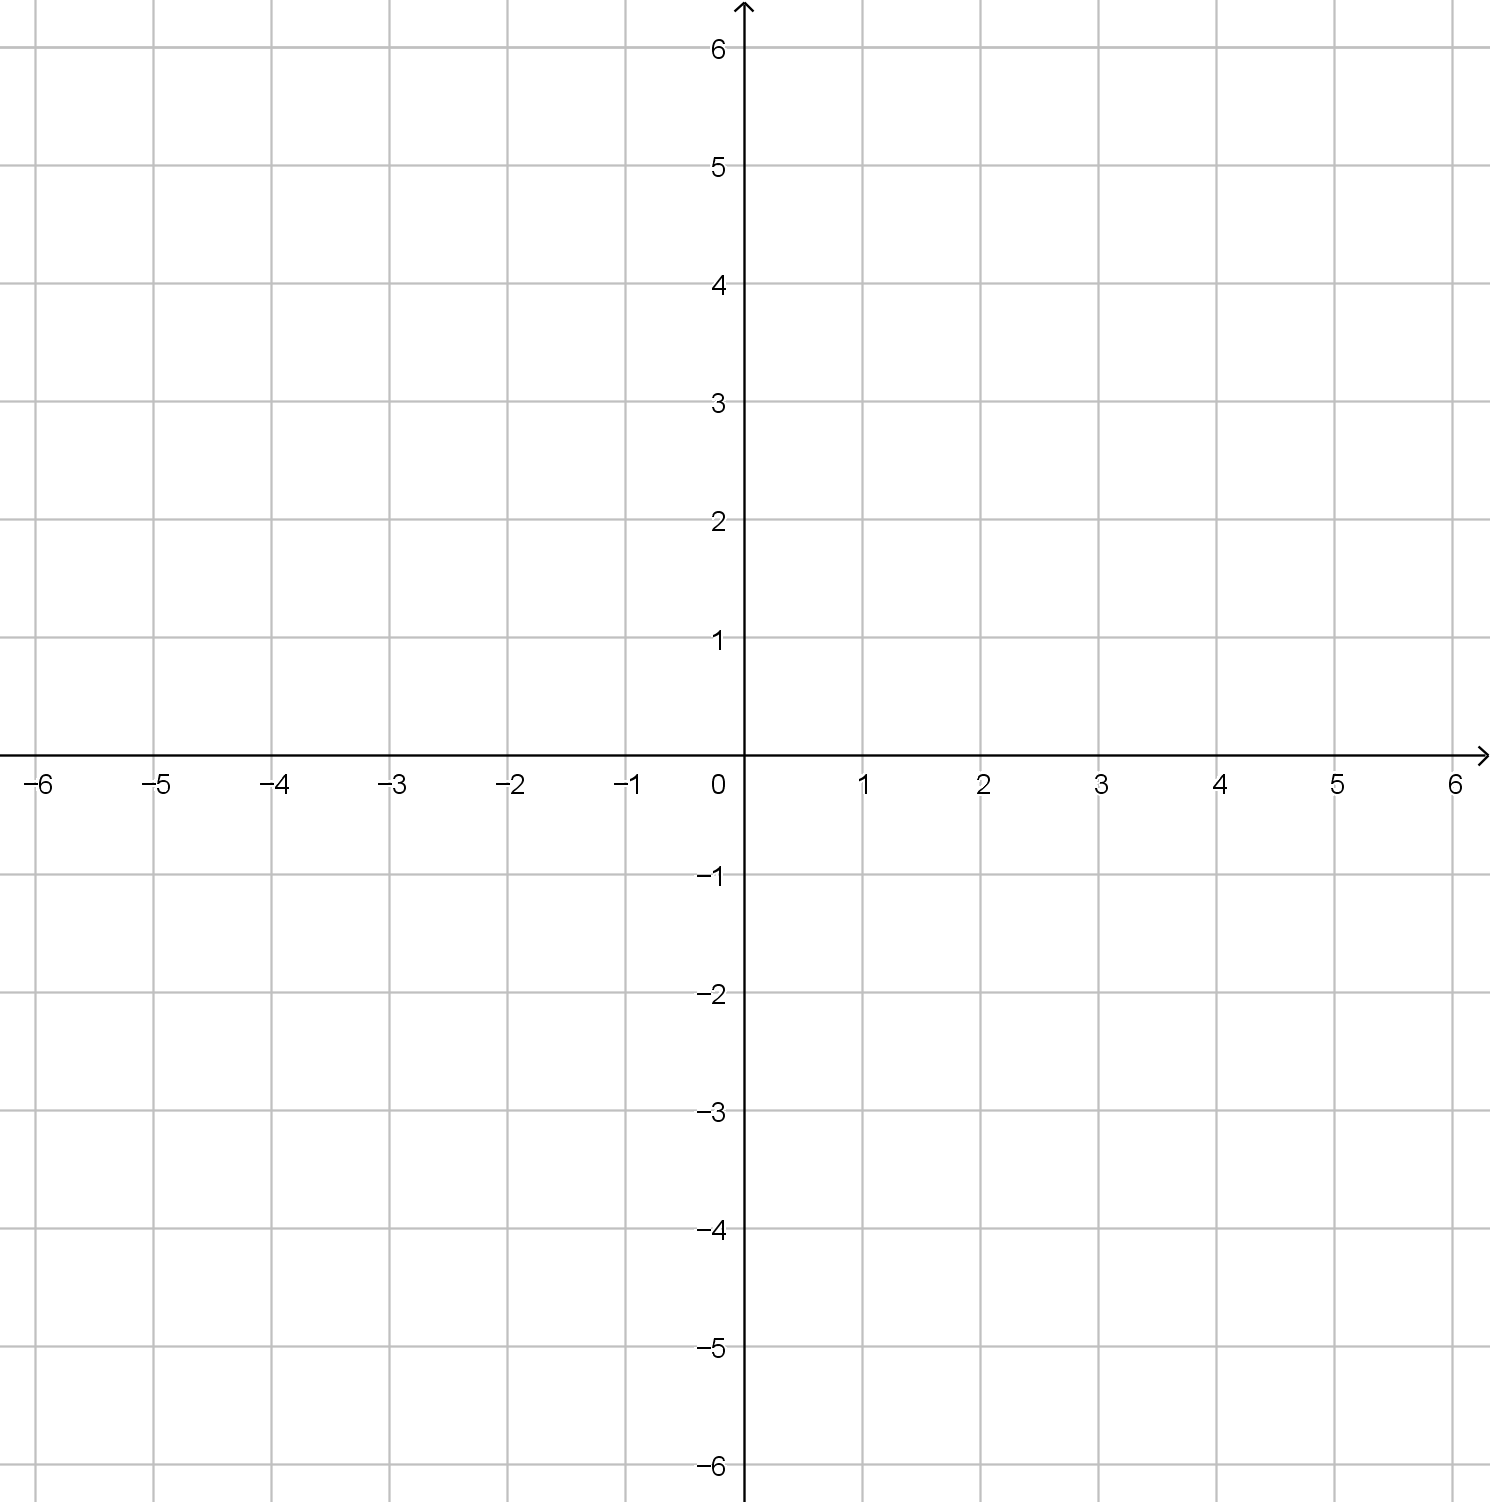
\includegraphics[width=0.8\textwidth]{66grid}
\end{center}

\begin{mdframed}
%
\theo{\(y=\frac kx\)의 그래프(\(k<0\))}
\begin{itemize}\label{rational6}
\item
대칭적인 곡선이다.
\item
제2사분면과 제4사분면에 그래프가 그려진다.
\item
\(|k|\)값이 커질수록 원점에서 멀어지고 \(|k|\)값이 작아질수록 원점에 가까워진다.
\end{itemize}
\end{mdframed}

%
\prob{함수 \(y=\frac kx\)의 정의역과 공역, 치역을 각각 말하여라.}\label{rational7}


\newpage
%
\exam{\(y=\frac{2x-5}{x-3}\)의 그래프를 그려라.}
\begin{mdframed}\label{rational8}
주어진 식의 좌변을 잘 정리하면
\[\frac{2x-5}{x-3}=\frac{2(x-3)+1}{x-3}=\frac1{x-3}+2\]
이다.
따라서 \(y=\frac1{x-3}+2\)의 그래프를 그리면 된다.\\
이 그래프는 \(y=\frac1x\)의 그래프를 \(x\)축의 방향으로 \(3\)만큼, \(y\)축의 방향으로 \(2\)만큼 평행이동시킨 그래프이다.
\begin{center}
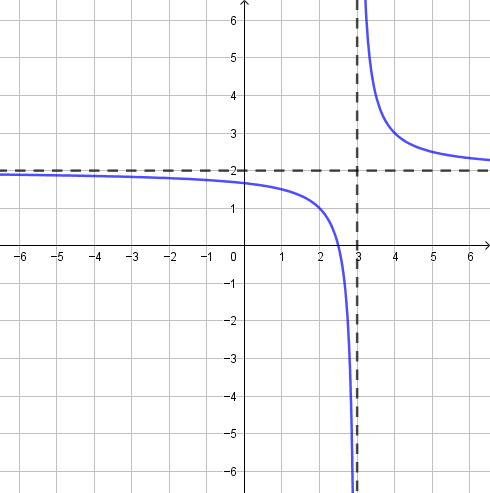
\includegraphics[width=0.85\textwidth]{rational_7}
\end{center}
이때, 곡선 위의 점들은 \(x\)의 절댓값이 커질수록 직선 \(y=2\)에 가까워지고 \(y\)의 절댓값이 커질수록 직선 \(x=3\)에 가까워진다.
이와 같은 두 직선 \(y=2\), \(x=3\)을 \fbox{점근선}이라고 부른다.

\bigskip
또한, 주어진 식 \(y=\frac{2x-5}{x-3}\)에 \(y=0\)을 대입하면 \(x=\frac52\)이고, \(x=0\)을 대입하면 \(y=\frac53\)이므로 \(x\)절편은 \(\frac52\), \(y\)절편은 \(\frac53\)이다.
\end{mdframed}

\newpage
%
\prob{}
다음 유리함수들의 그래프를 그리고 점근선과 \(x\)절편, \(y\)절편을 구하여라.\label{rational9}
\par\bigskip\noindent
(1)\:\:\(y=\frac{3x+5}{x+1}\)
\begin{center}
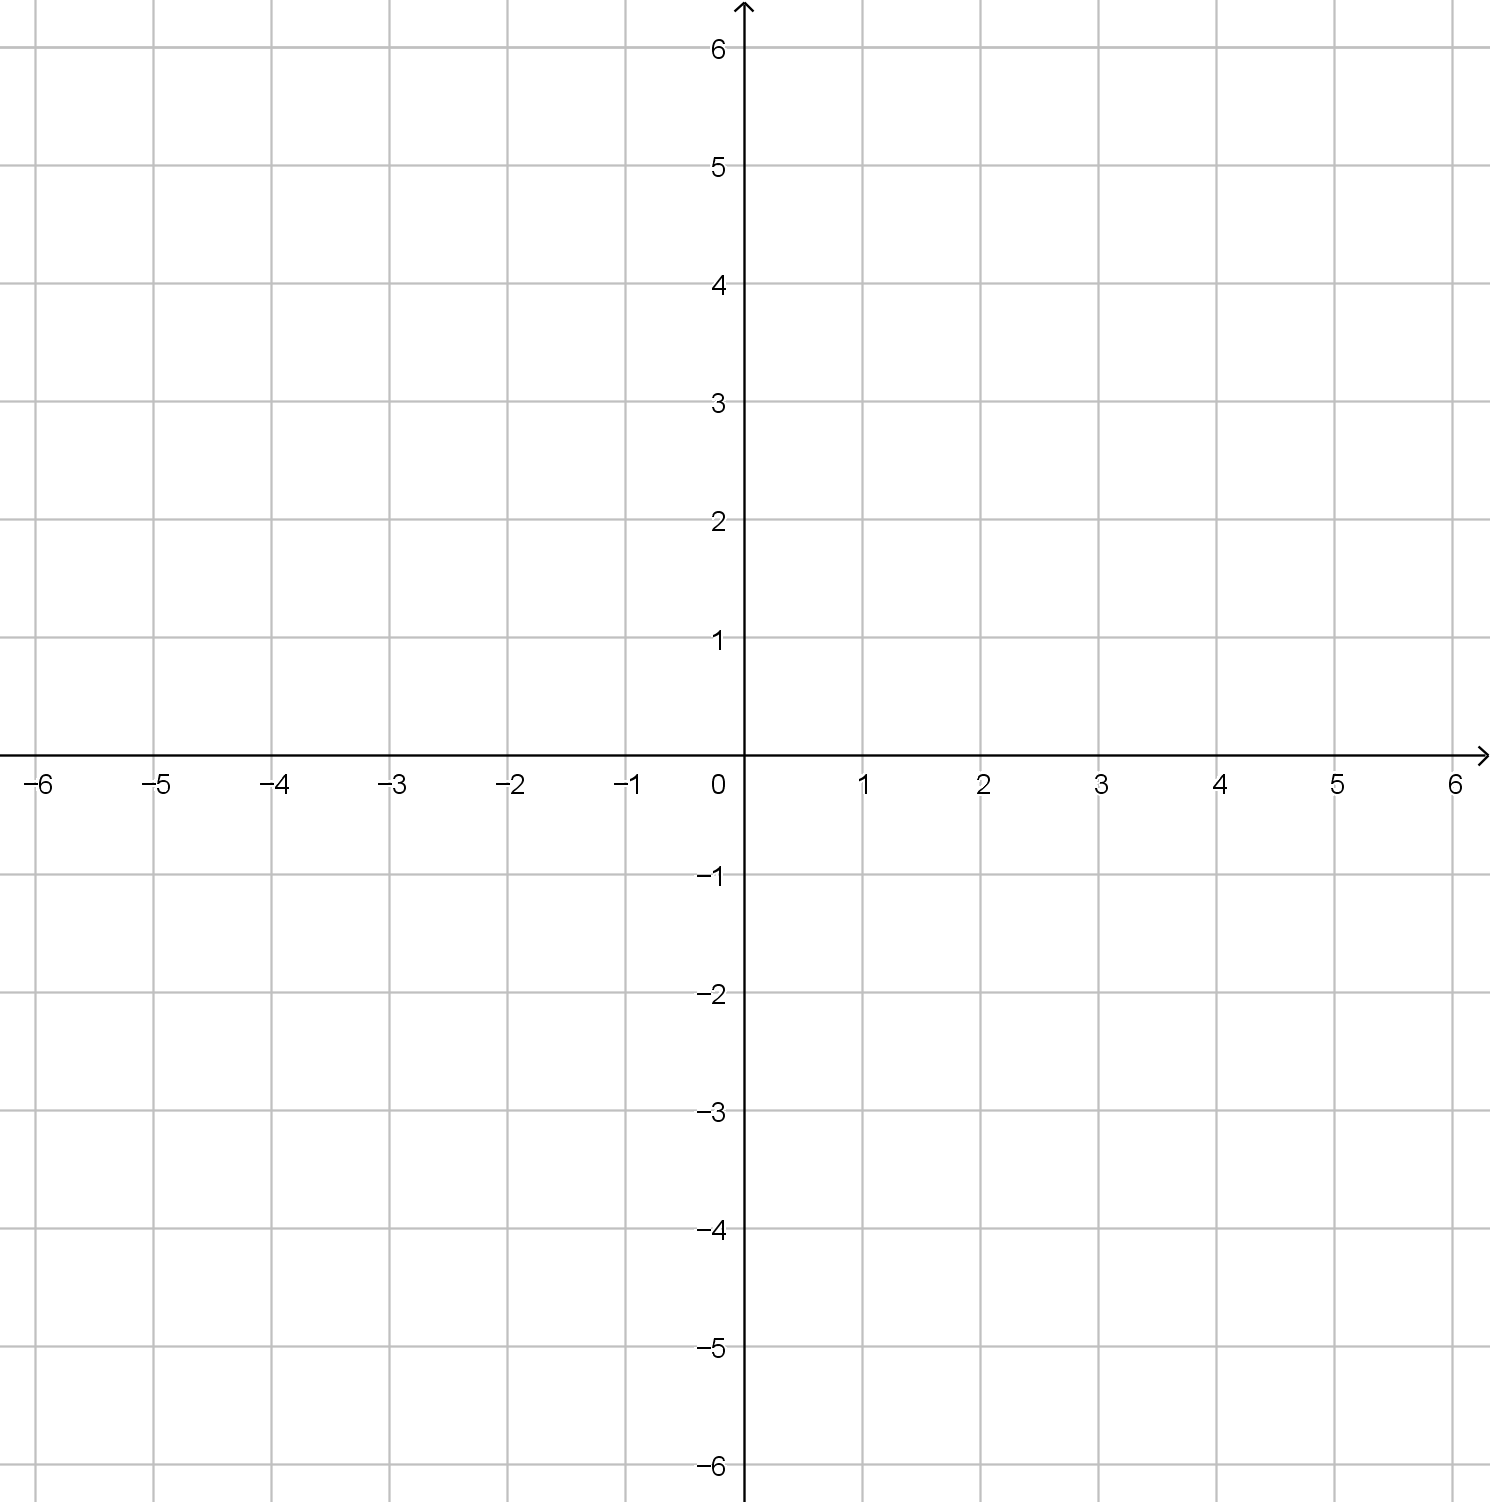
\includegraphics[width=0.8\textwidth]{66grid}
\end{center}
\hspace{0.65\textwidth}\parbox[t]{0.3\textwidth}{점근선 :\\[20pt]\(x\)절편 \(=\)\\[20pt]\(y\)절편 \(=\)}
\newpage
(2)\:\:\(y=\frac{2x}{x-2}\)
\begin{center}
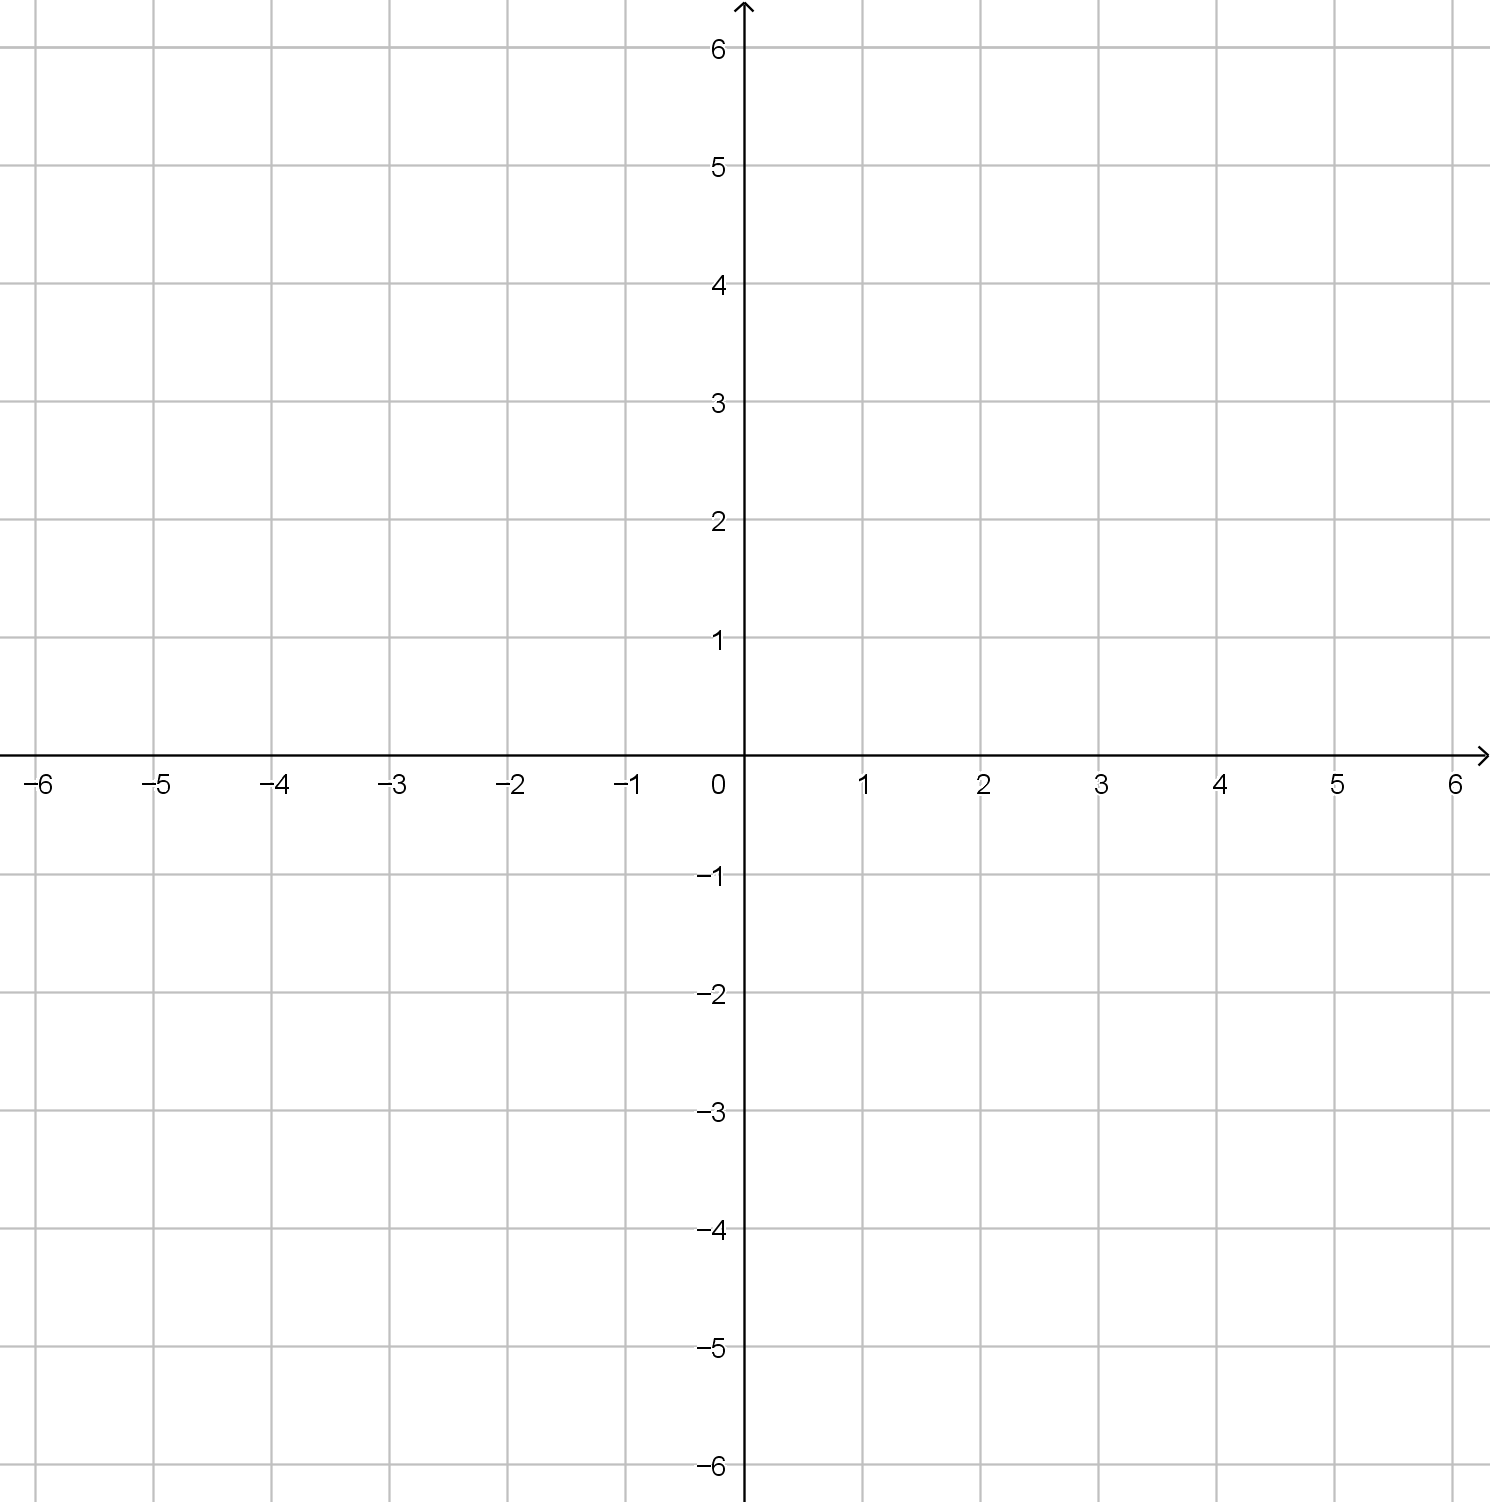
\includegraphics[width=0.8\textwidth]{66grid}
\end{center}
\hspace{0.65\textwidth}\parbox[t]{0.3\textwidth}{점근선 :\\[20pt]\(x\)절편 \(=\)\\[20pt]\(y\)절편 \(=\)}
\newpage
(3)\:\:\(y=\frac{-x+2}{x-3}\)
\begin{center}
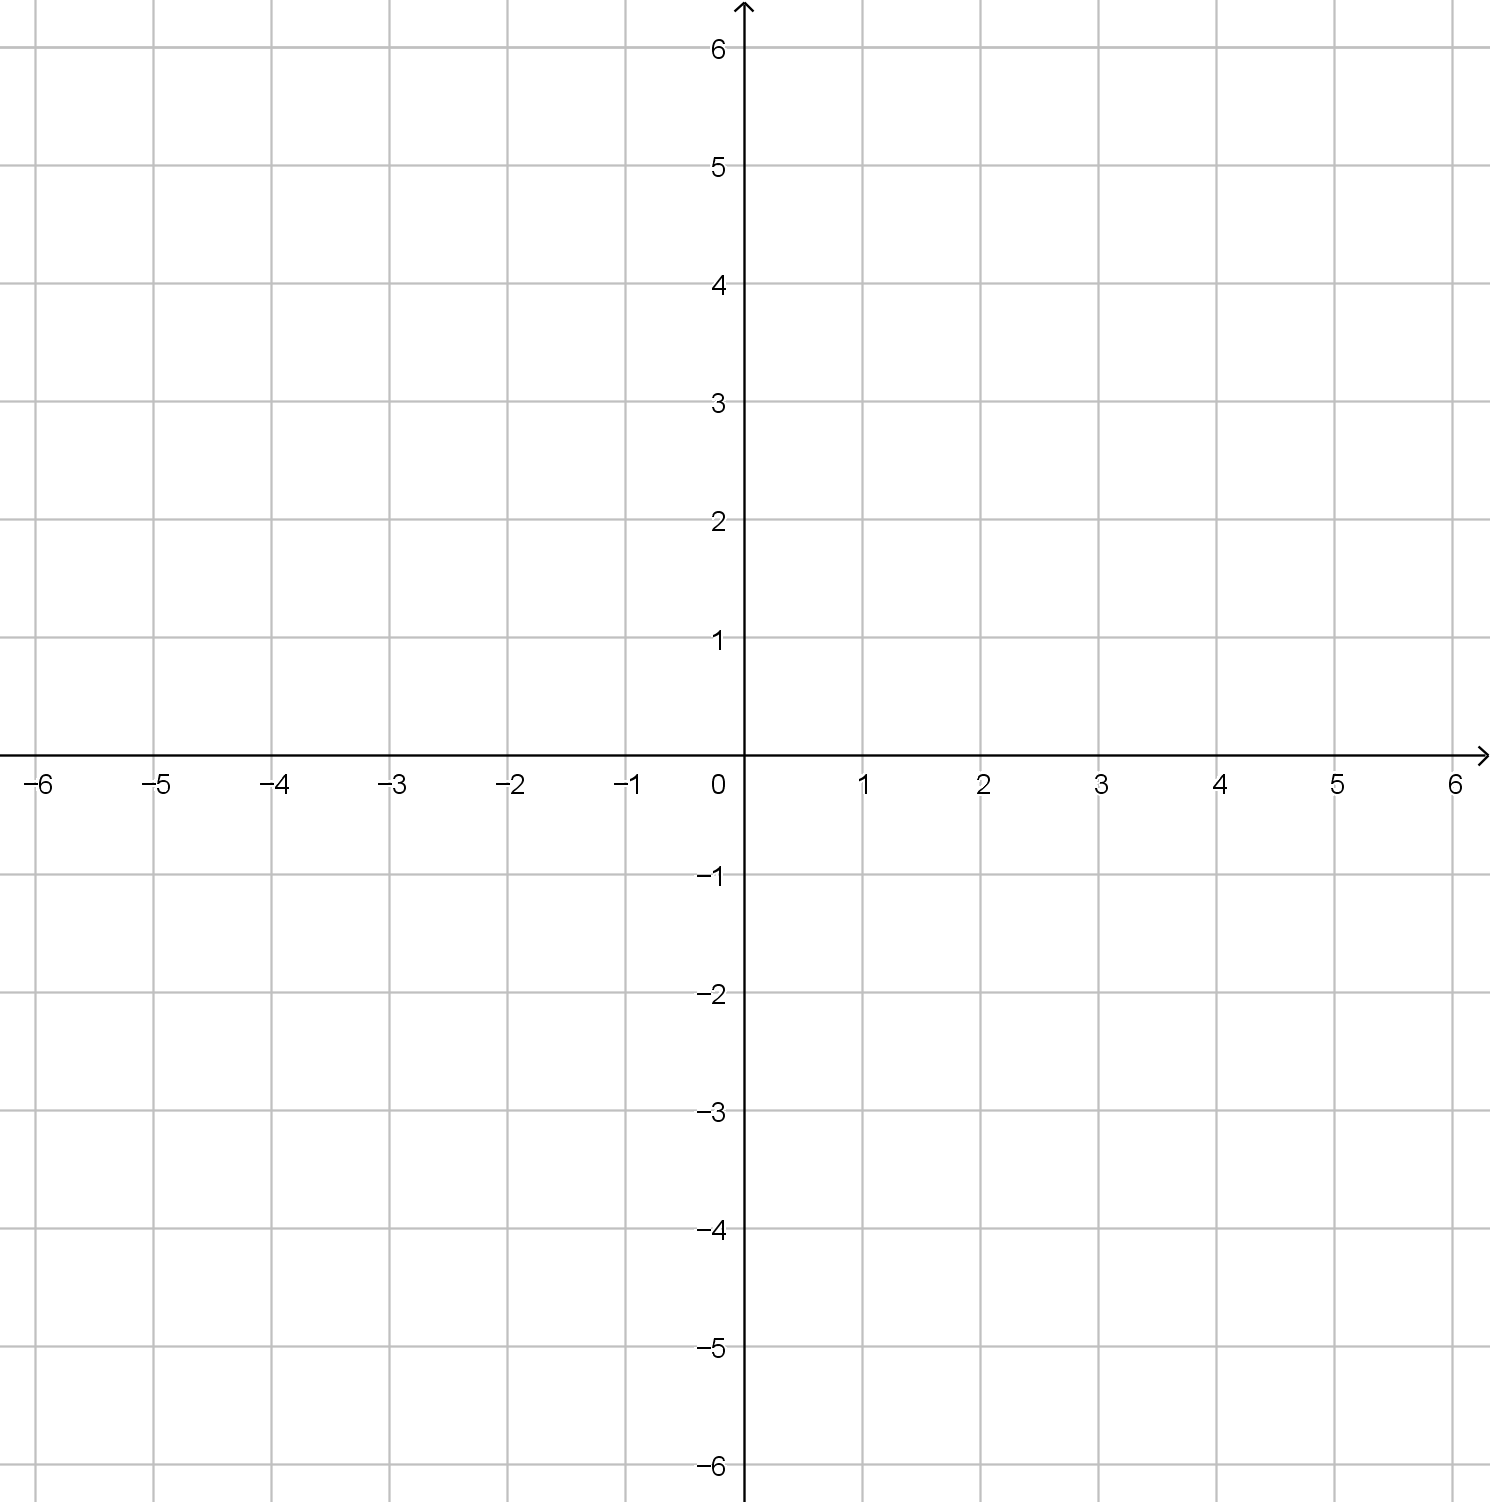
\includegraphics[width=0.8\textwidth]{66grid}
\end{center}
\hspace{0.65\textwidth}\parbox[t]{0.3\textwidth}{점근선 :\\[20pt]\(x\)절편 \(=\)\\[20pt]\(y\)절편 \(=\)}

%%
\section{무리함수의 그래프}

%%%%%%%alternative way


%
\exam{\(y=\sqrt x\)의 그래프를 그려라.}\label{irrational1}
\(y=\sqrt x\)를 만족시키는 모든 점 \((x,y)\)를 표시하면 된다.
\[(x,y)=(0,0),(1,1),(4,2),(9,3),\cdots\]
등을 좌표평면에 표시하고 자연스럽게 이으면
\begin{center}
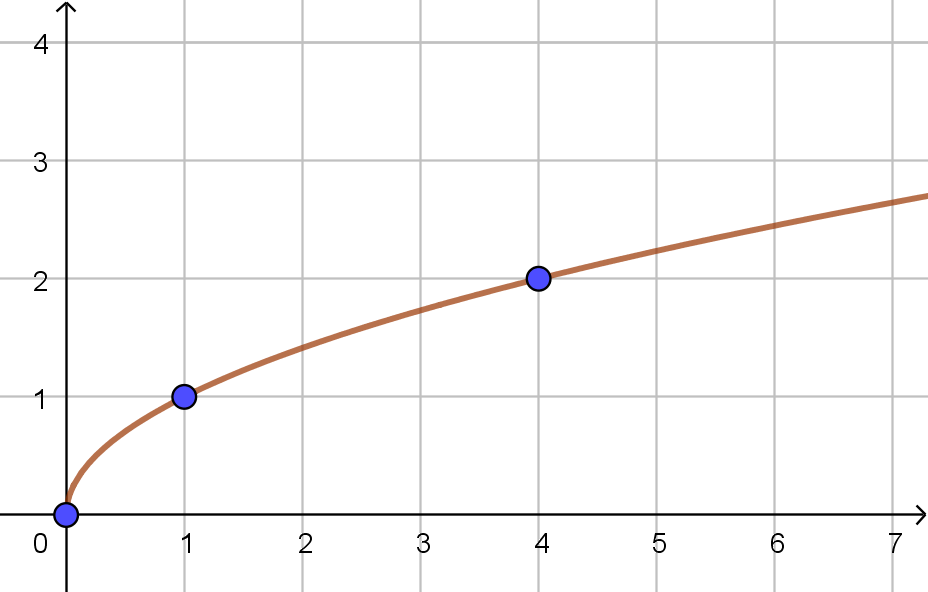
\includegraphics[width=0.5\textwidth]{irrational_1}
\end{center}
이 된다.

\bigskip
잘 살펴보면 \(y=\sqrt x\)의 그래프는 \(y=x^2\)의 그래프와 비슷하게 생겼다.
\(y=x^2\)의 그래프 중 제1사분면 부분을 \(y=x\)에 대해 대칭이동시키면 \(y=\sqrt x\)의 그래프가 되는 것이다.

실제로 함수 \(y=x^2\)의 정의역이 \(\{x\ba x\ge0\}\)이고 공역이 \(\{y\ba y\ge 0\}\)이라고 가정하고, 이 함수의 역함수를 구해보면,
\[y=x^2\qquad(x\ge0,\,y\ge0)\]
에서 \(x\)대신에 \(y\)를, \(y\)대신에 \(x\)를 대입시켜야 하므로
\[x=y^2\qquad(y\ge0,\,x\ge0)\]
이고 \(y\ge0\)로부터
\[y=\sqrt x\qquad(x\ge0,\,y\ge0)\]
이다.
즉, \(A\)를 음이 아닌 실수들의 집합이라고 할 때, %=\{x\ba x\ge0\}\)일 때, 
함수 \(f:A\to A\), \(f(x)=x^2\)의 역함수 \(f^{-1}:A\to A\)는 \(f^{-1}(x)=\sqrt x\)이다.

\newpage
%
\exam{다음 무리함수들의 그래프를 그려라.}
\begin{enumerate}\label{irrational2}
\item
\(y=-\sqrt x\)
\item
\(y=\sqrt{-x}\)
\item
\(y=-\sqrt{-x}\)
\end{enumerate}
\begin{mdframed}
(1)의 경우 식 \(y=\sqrt x\)에 \(y\)대신 \(-y\)를 대입한 \(-y=\sqrt x\)를 정리하여 얻어질 수 있다.
\[y=\sqrt x
\quad\xrightarrow[y\:\leftarrow\: -y\:\:대입]{x축\:\:대칭}\quad
y=-\sqrt x\]
따라서 \(y=-\sqrt x\)의 그래프는 \(y=\sqrt x\)의 그래프를 \(y\)축대칭시킨 것이다.
(2)와 (3)의 경우에는
\begin{gather*}
y=\sqrt x
\quad\xrightarrow[x\:\leftarrow\: -x\:\:대입]{y축\:\:대칭}\quad
y=\sqrt{-x}
\\[10pt]
y=\sqrt x
\quad\xrightarrow[x\:\leftarrow\: -x,\quad y\:\leftarrow\: -y\:\:대입]{원점\:\:대칭}\quad
y=-\sqrt{-x}
\end{gather*}
이다.
따라서 \(y=\sqrt{-x}\)와 \(y=-\sqrt{-x}\)의 그래프는 \(y=\sqrt x\)의 그래프를 각각 \(x\)축대칭, 원점대칭시켜 얻어진다.
이것들을 좌표평면 위에 그리면 다음과 같다.
\begin{center}
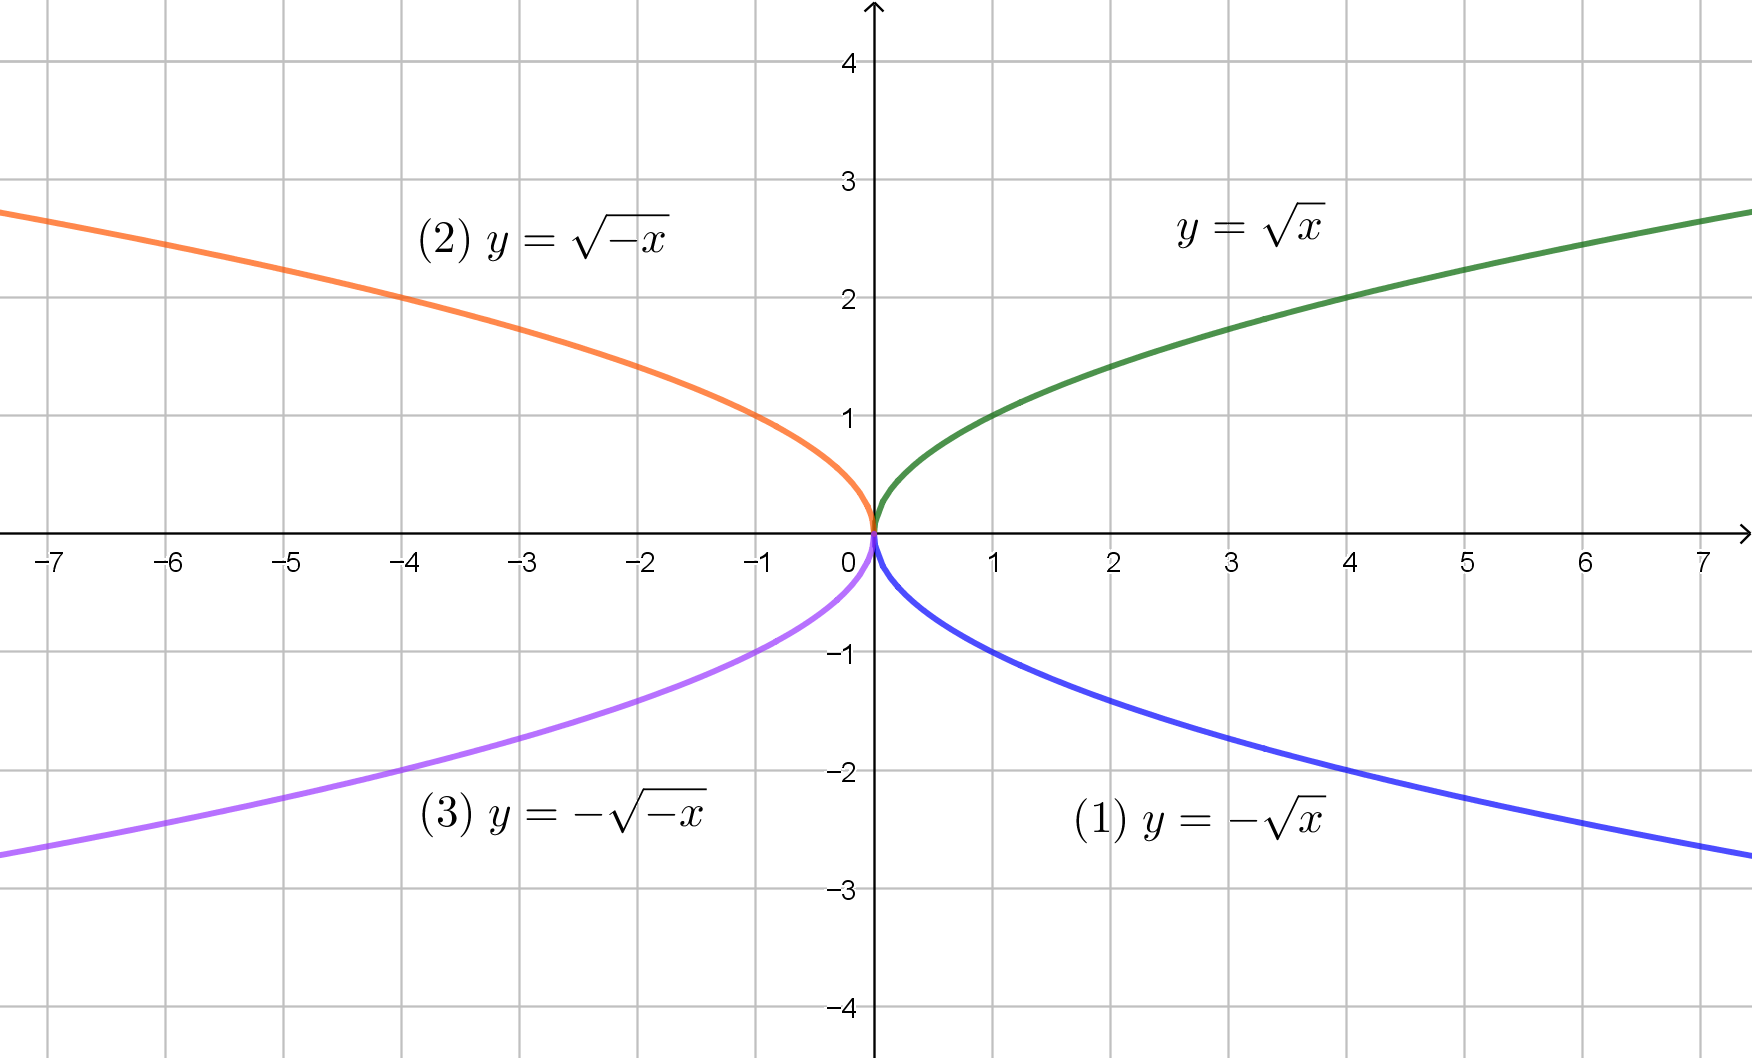
\includegraphics[width=0.99\textwidth]{irrational_2}
\end{center}
\end{mdframed}

\newpage
%
\exam{\(y=-\sqrt{2x}\)의 그래프를 그려라.}\label{irrational3}
\begin{mdframed}
\(y=-\sqrt{2x}\)의 그래프의 개형은 \(y=-\sqrt x\)의 그래프와 비슷할 것이다.
\((0,0)\), \((2,-2)\) 등을 지나도록 그래프를 그리면 다음과 같다.
\begin{center}
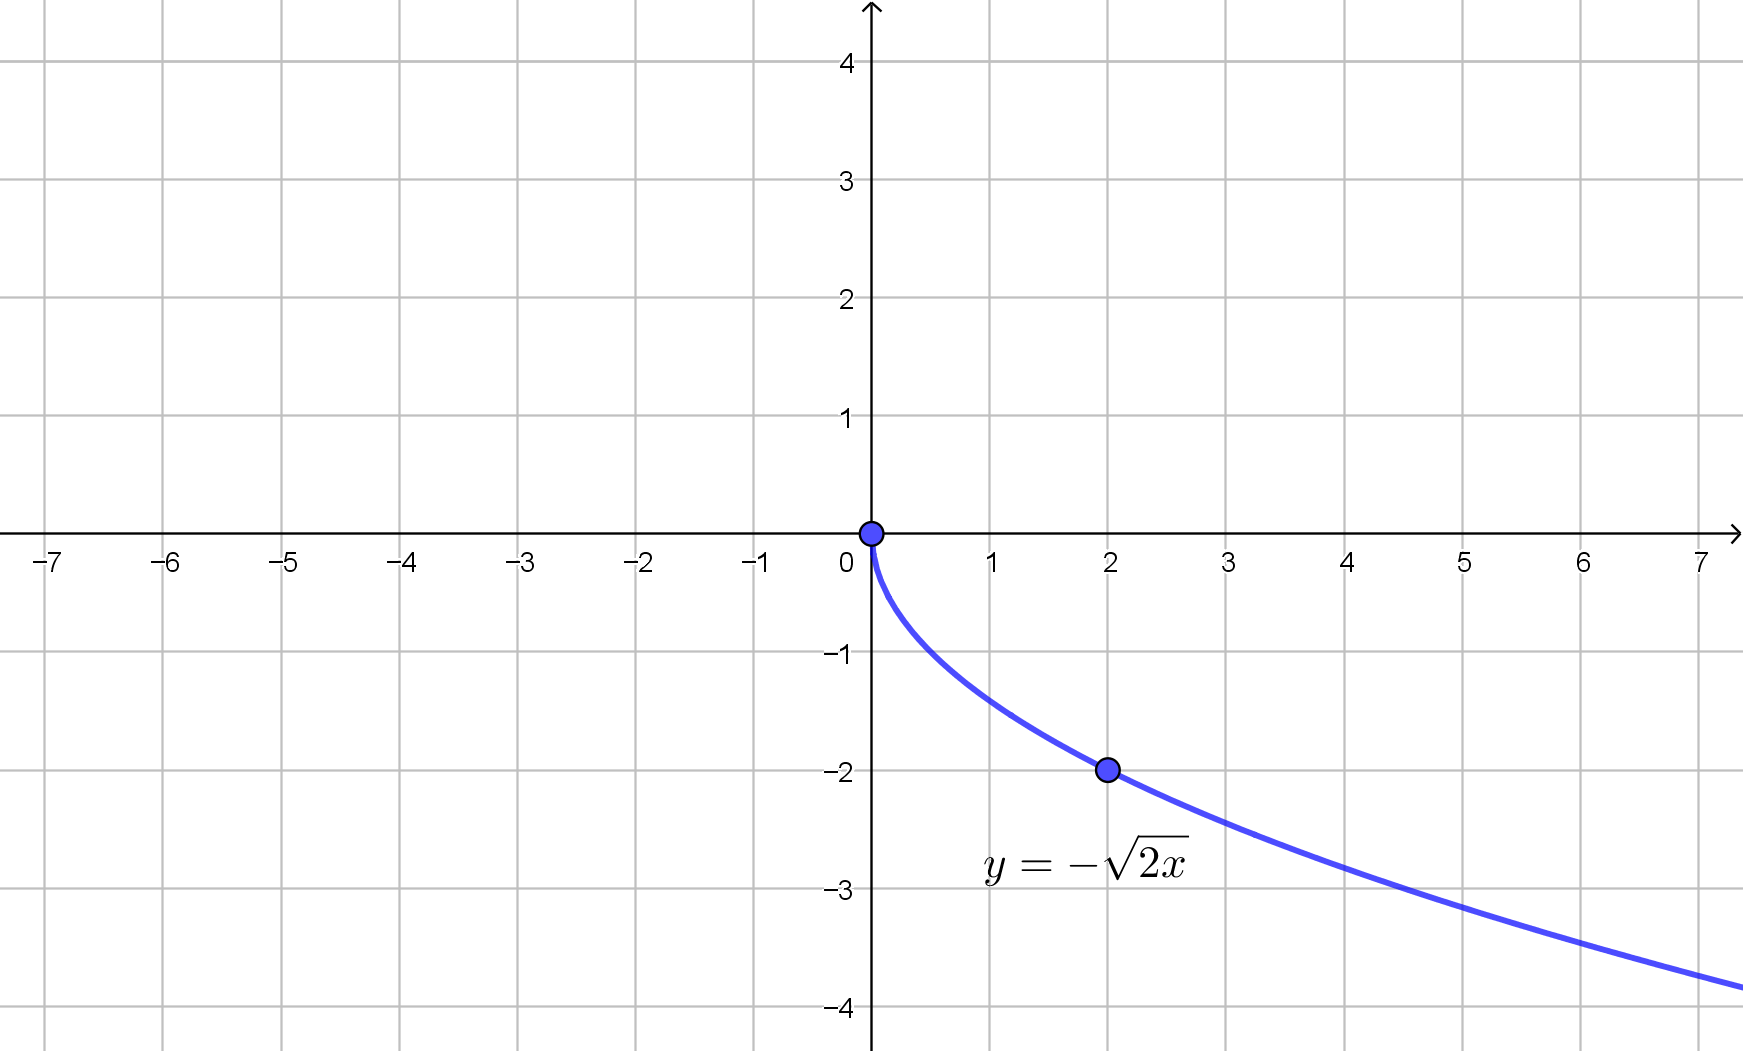
\includegraphics[width=0.99\textwidth]{irrational_3}
\end{center}
\end{mdframed}

%
\prob{다음 무리함수들의 그래프를 그려라.}\label{irrational4}
(1)\:\:\(y=\sqrt{-\frac12x}\)
\begin{center}
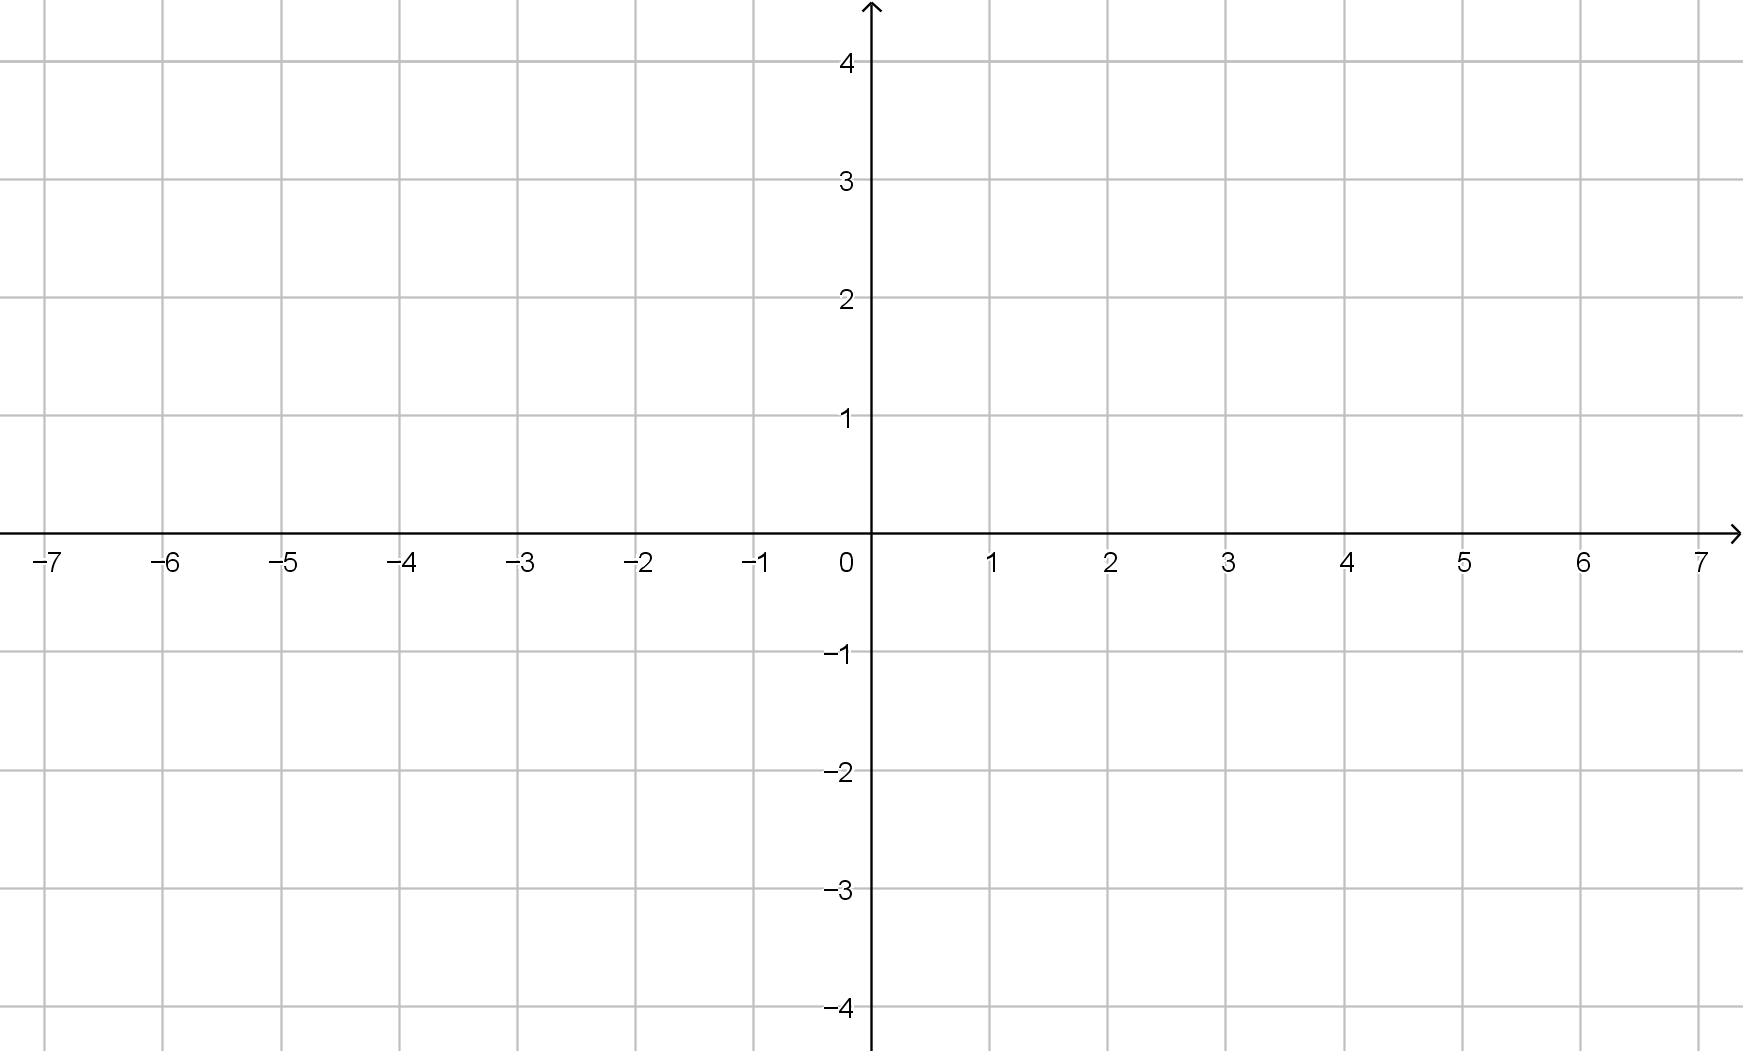
\includegraphics[width=0.99\textwidth]{74grid}
\end{center}
\newpage
(2)\:\:\(y=-\sqrt{-3x}\)
\begin{center}
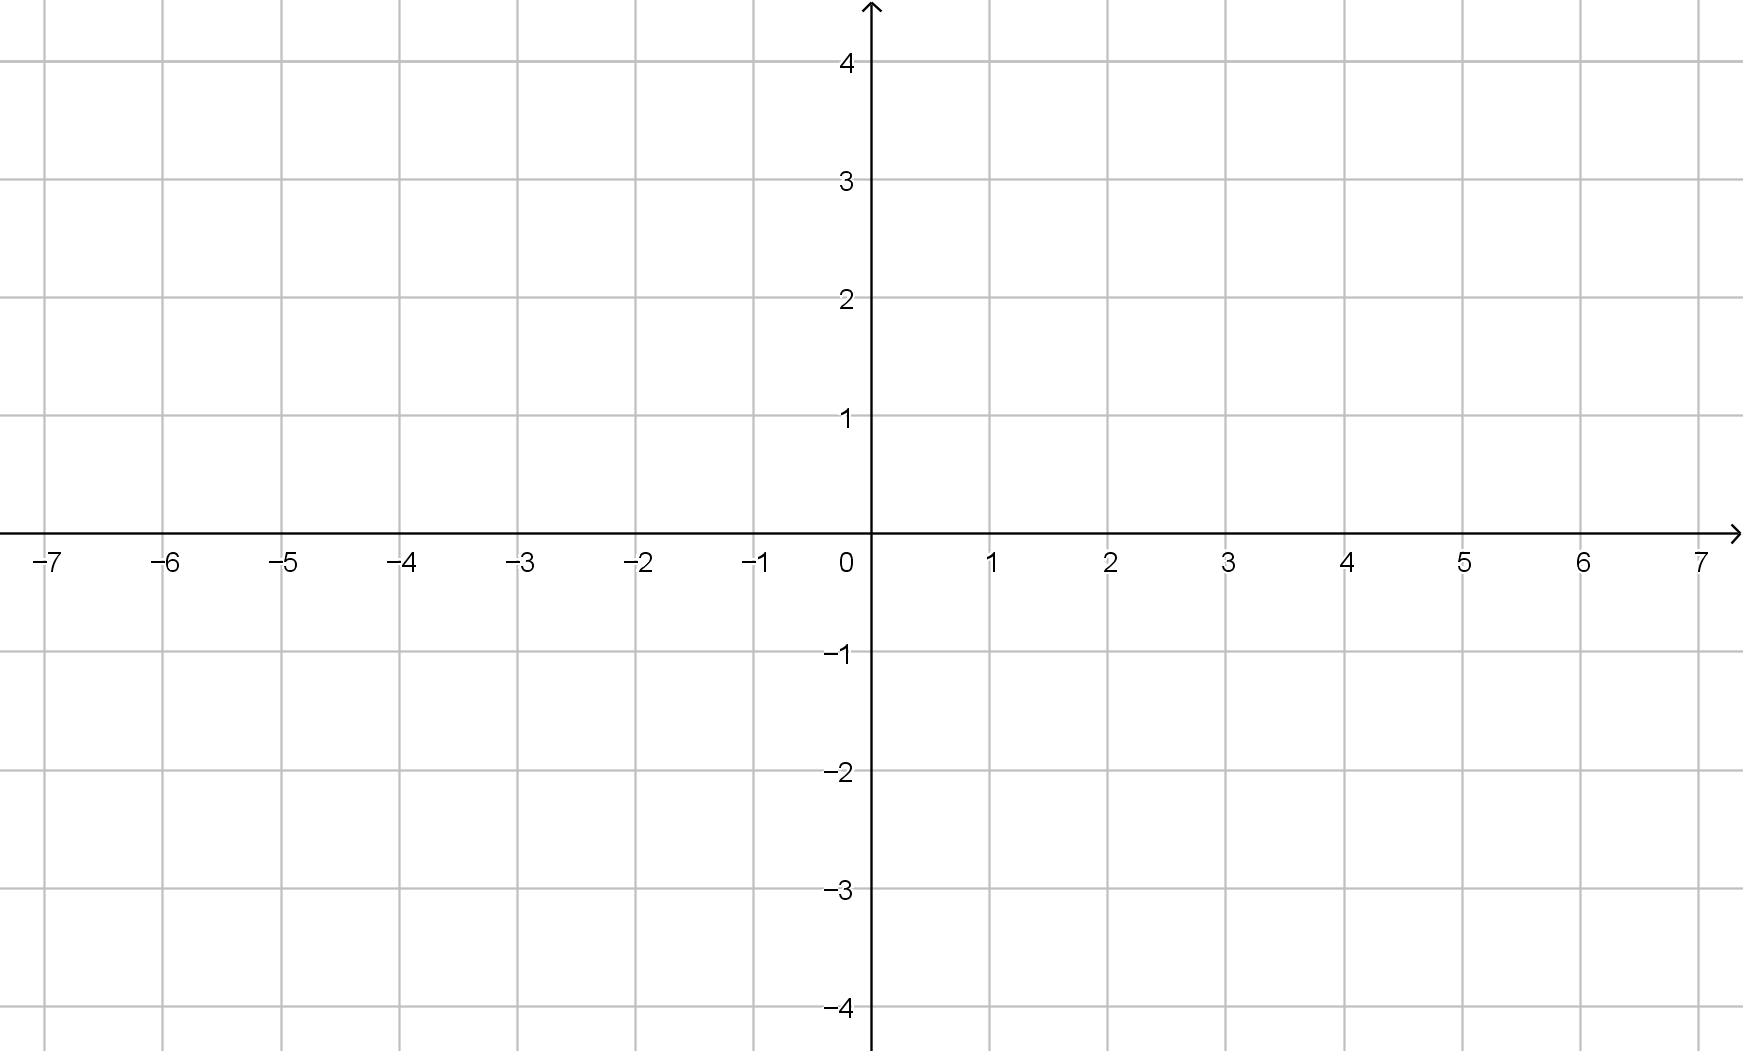
\includegraphics[width=0.99\textwidth]{74grid}
\end{center}

%
\prob{}\label{irrational5}
예시 \ref{irrational3})과 문제 \ref{irrational4})의 세 함수들의 정의역과 치역을 각각 말하여라.
\begin{center}
\begin{tabu}to.7\textwidth[tabulinesep=10pt]{X|X[c]|X[c]}
					&정의역			&치역\\\hline
\(y=-\sqrt{2x}\)			&\(\{x\ba x\ge0\}\)	&\(\{y\ba y\le0\}\)\\
\(y=\sqrt{-\frac12x}\)	&\\
\(y=-\sqrt{-3x}\)		&
\end{tabu}
\end{center}

\newpage
%
\exam{\(y=-\sqrt{2x+4}+1\)의 그래프를 그리고, \(x\)절편과 \(y\)절편을 각각 구하여라.}
\begin{mdframed}\label{irrational6}
주어진 식을 잘 정리하면
\[y-1=-\sqrt{2(x+2)}\]
가 된다.
따라서 이 함수의 그래프는 \(y=-\sqrt{2x}\)의 그래프를\\
\(x\)축의 방향으로 \(-2\)만큼, \(y\)축의 방향으로 \(1\)만큼 평행이동시킨 것이다.\\
\(y=-\sqrt{2x}\)의 그래프가 \((0,0)\), \((2,-2)\)를 지나기 때문에\\
\(y=-\sqrt{2x+4}+1\)의 그래프는 \((-2,1)\), \((0,-1)\)을 지난다.
\begin{center}
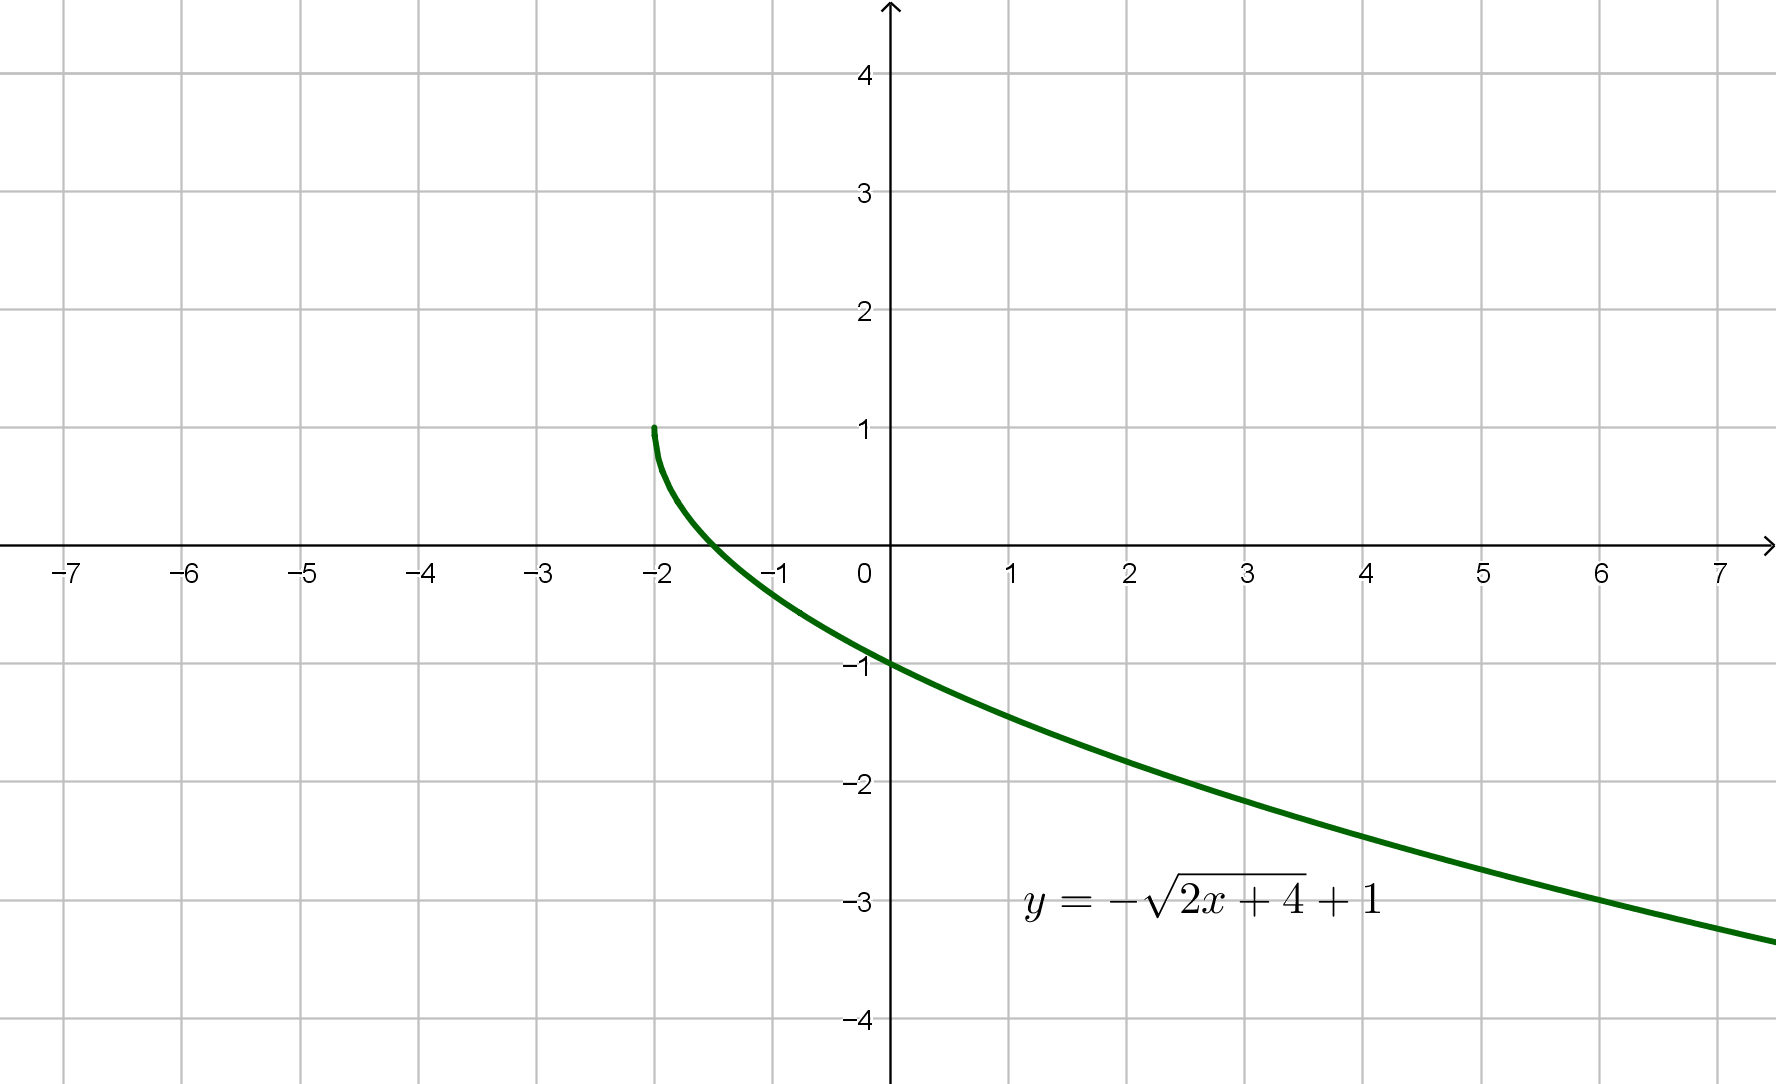
\includegraphics[width=0.99\textwidth]{irrational_6}
\end{center}
이다.

\bigskip
또한, 주어진 식 \(y=-\sqrt{2x+4}+1\)에\\[10pt]
\(y=0\)을 대입하면 \(x=-\frac32\)이고, \(x=0\)을 대입하면 \(y=-1\)이므로\\[10pt]
\(x\)절편은 \(-\frac32\), \(y\)절편은 \(-1\)이다.
\end{mdframed}

\newpage
%
\prob{}
다음 무리함수들의 그래프를 그리고 \(x\)절편, \(y\)절편을 구하여라.\label{irrational7}
\par\bigskip\noindent
(1)\:\:\(y=\sqrt{-\frac12x+3}\)
\begin{center}
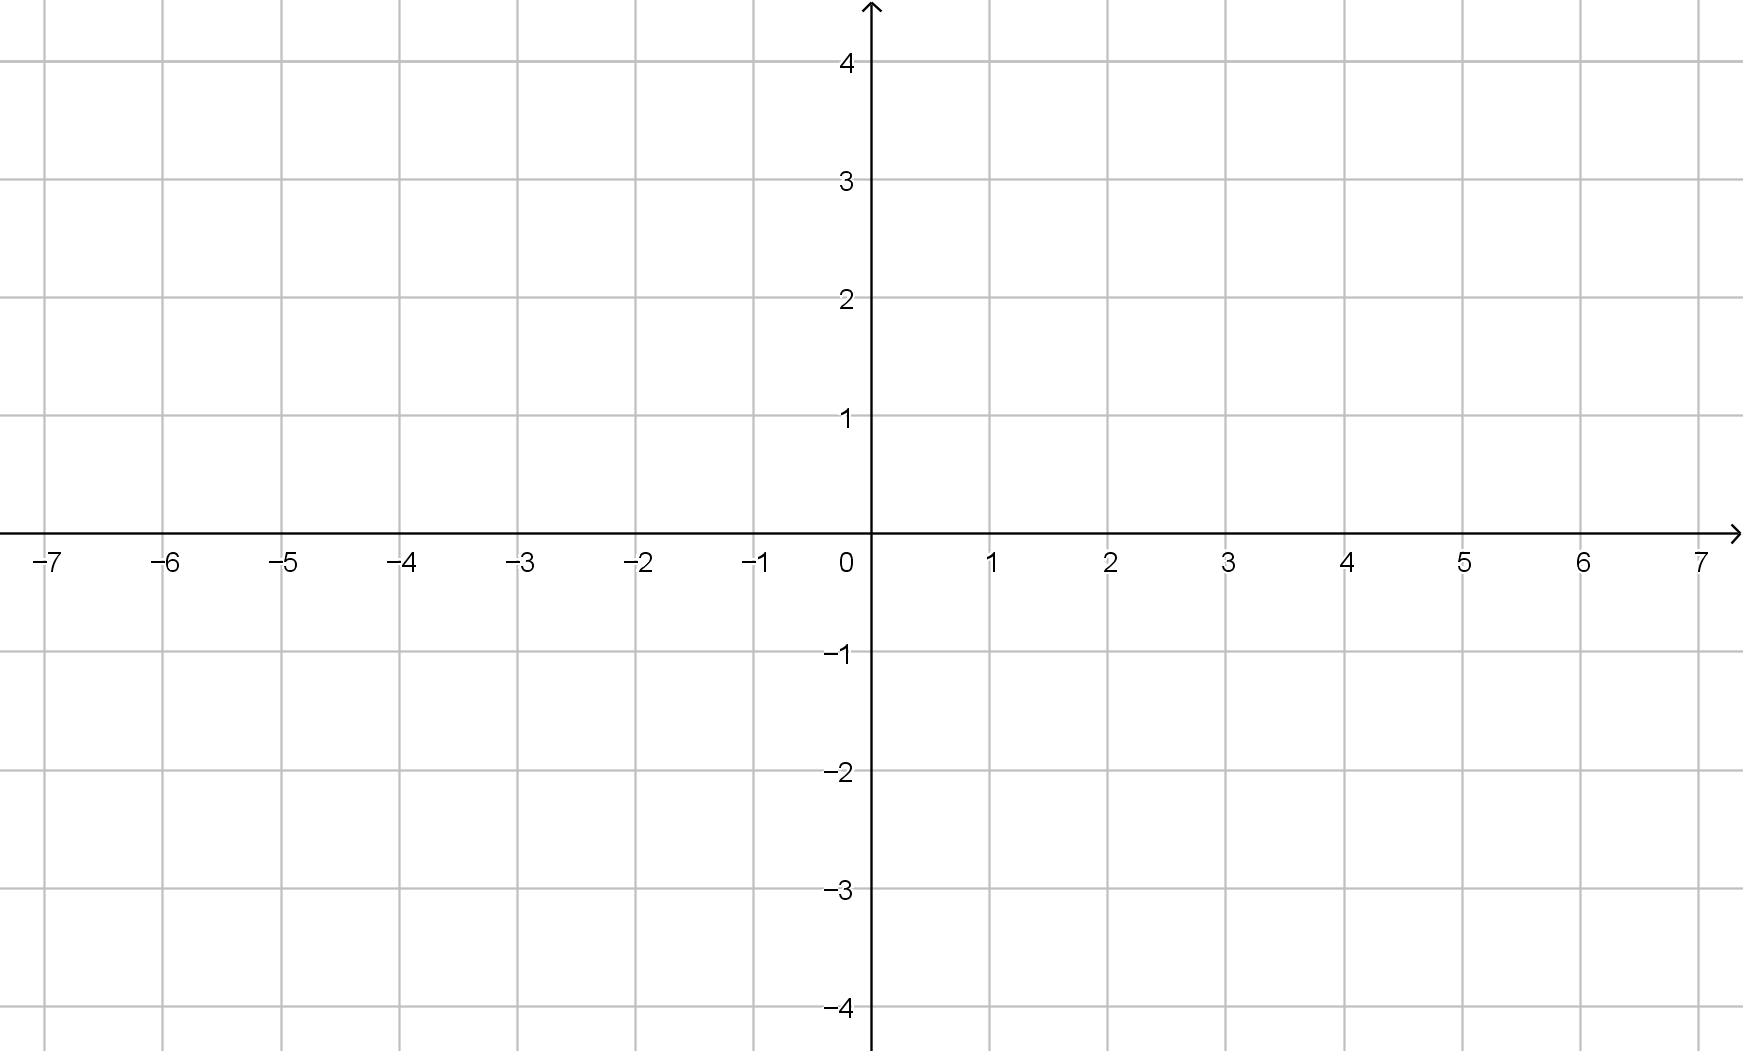
\includegraphics[width=0.8\textwidth]{74grid}
\end{center}
\hspace{0.65\textwidth}\parbox[t]{0.3\textwidth}{\(x\)절편 \(=\)\\\(y\)절편 \(=\)}

(2)\:\:\(y=-\sqrt{-3x+9}+3\)
\begin{center}
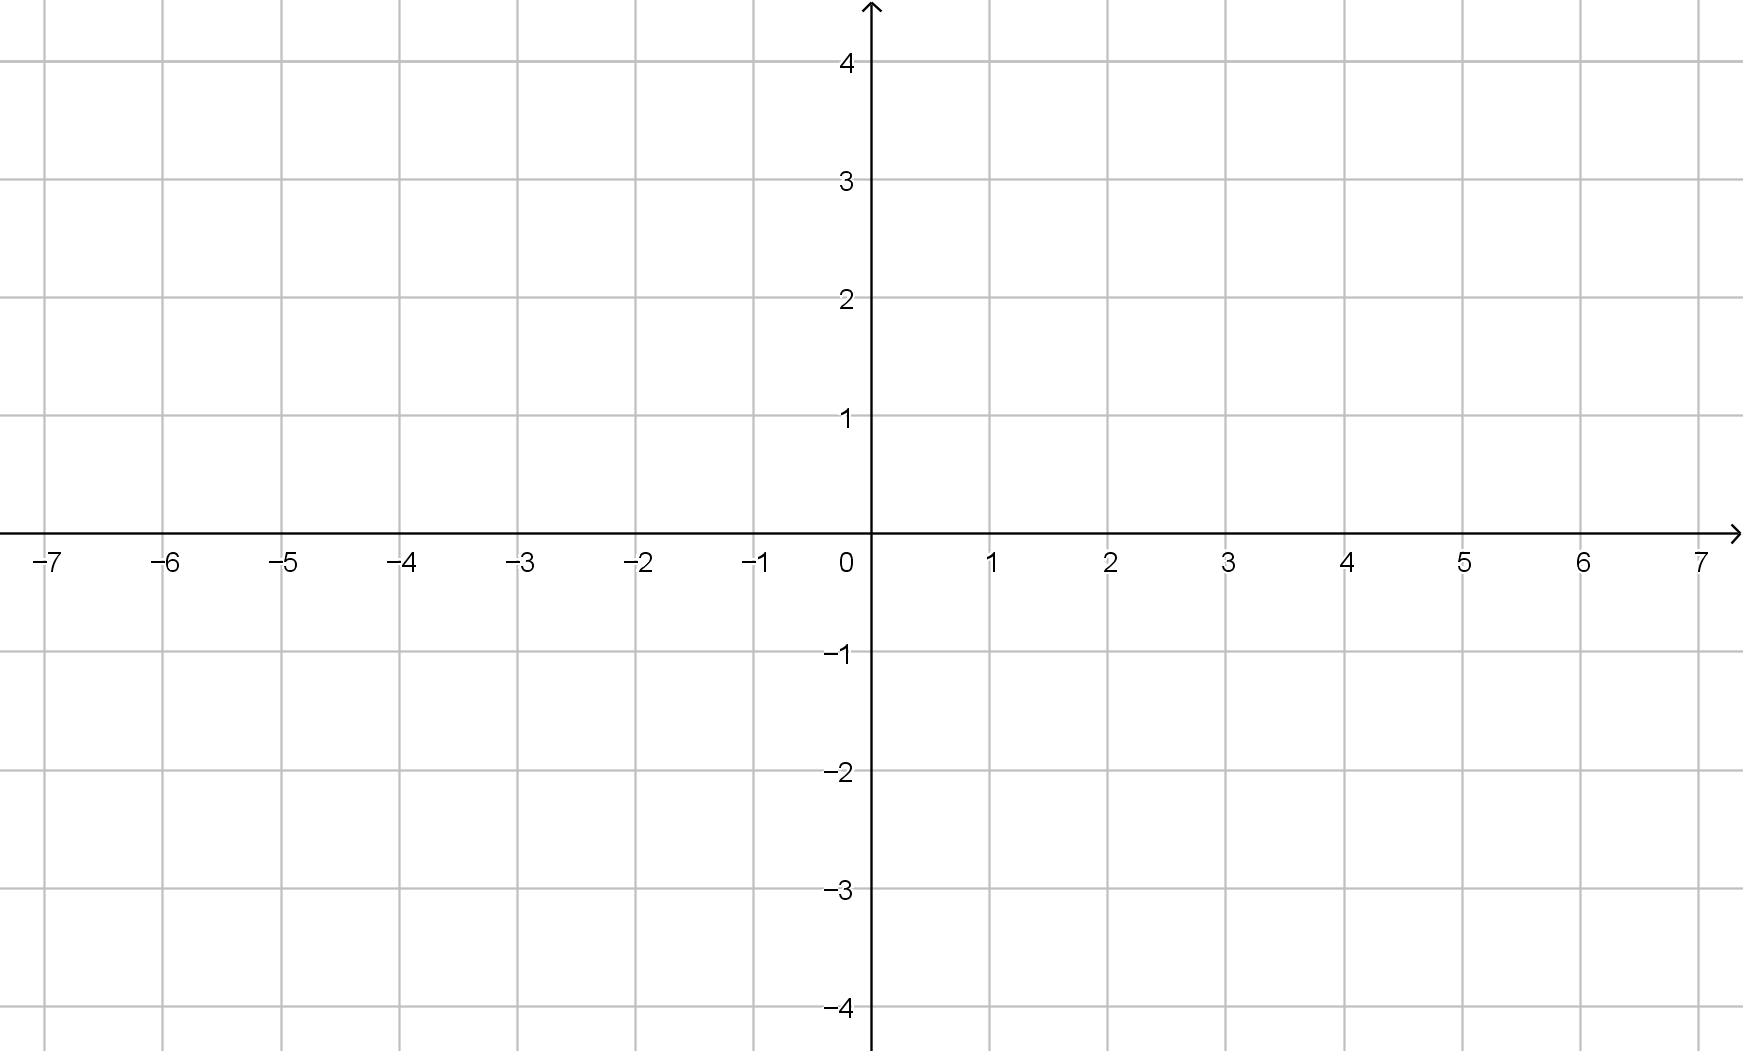
\includegraphics[width=0.8\textwidth]{74grid}
\end{center}
\hspace{0.65\textwidth}\parbox[t]{0.3\textwidth}{\(x\)절편 \(=\)\\\(y\)절편 \(=\)}

%%
\section*{답}
\addcontentsline{toc}{chapter}{\protect\numberline{*}답}
\begin{multicols*}{2}
%
\an{review3}
\(y=3x-5\)

%
\an{review6}
\begin{enumerate}
\item
\((x+3)^2+(y+1)^2=1\)
\item
\((x-1)^2+(y-3)^2=1\)
\end{enumerate}

%
\an{rational2}
\begin{center}
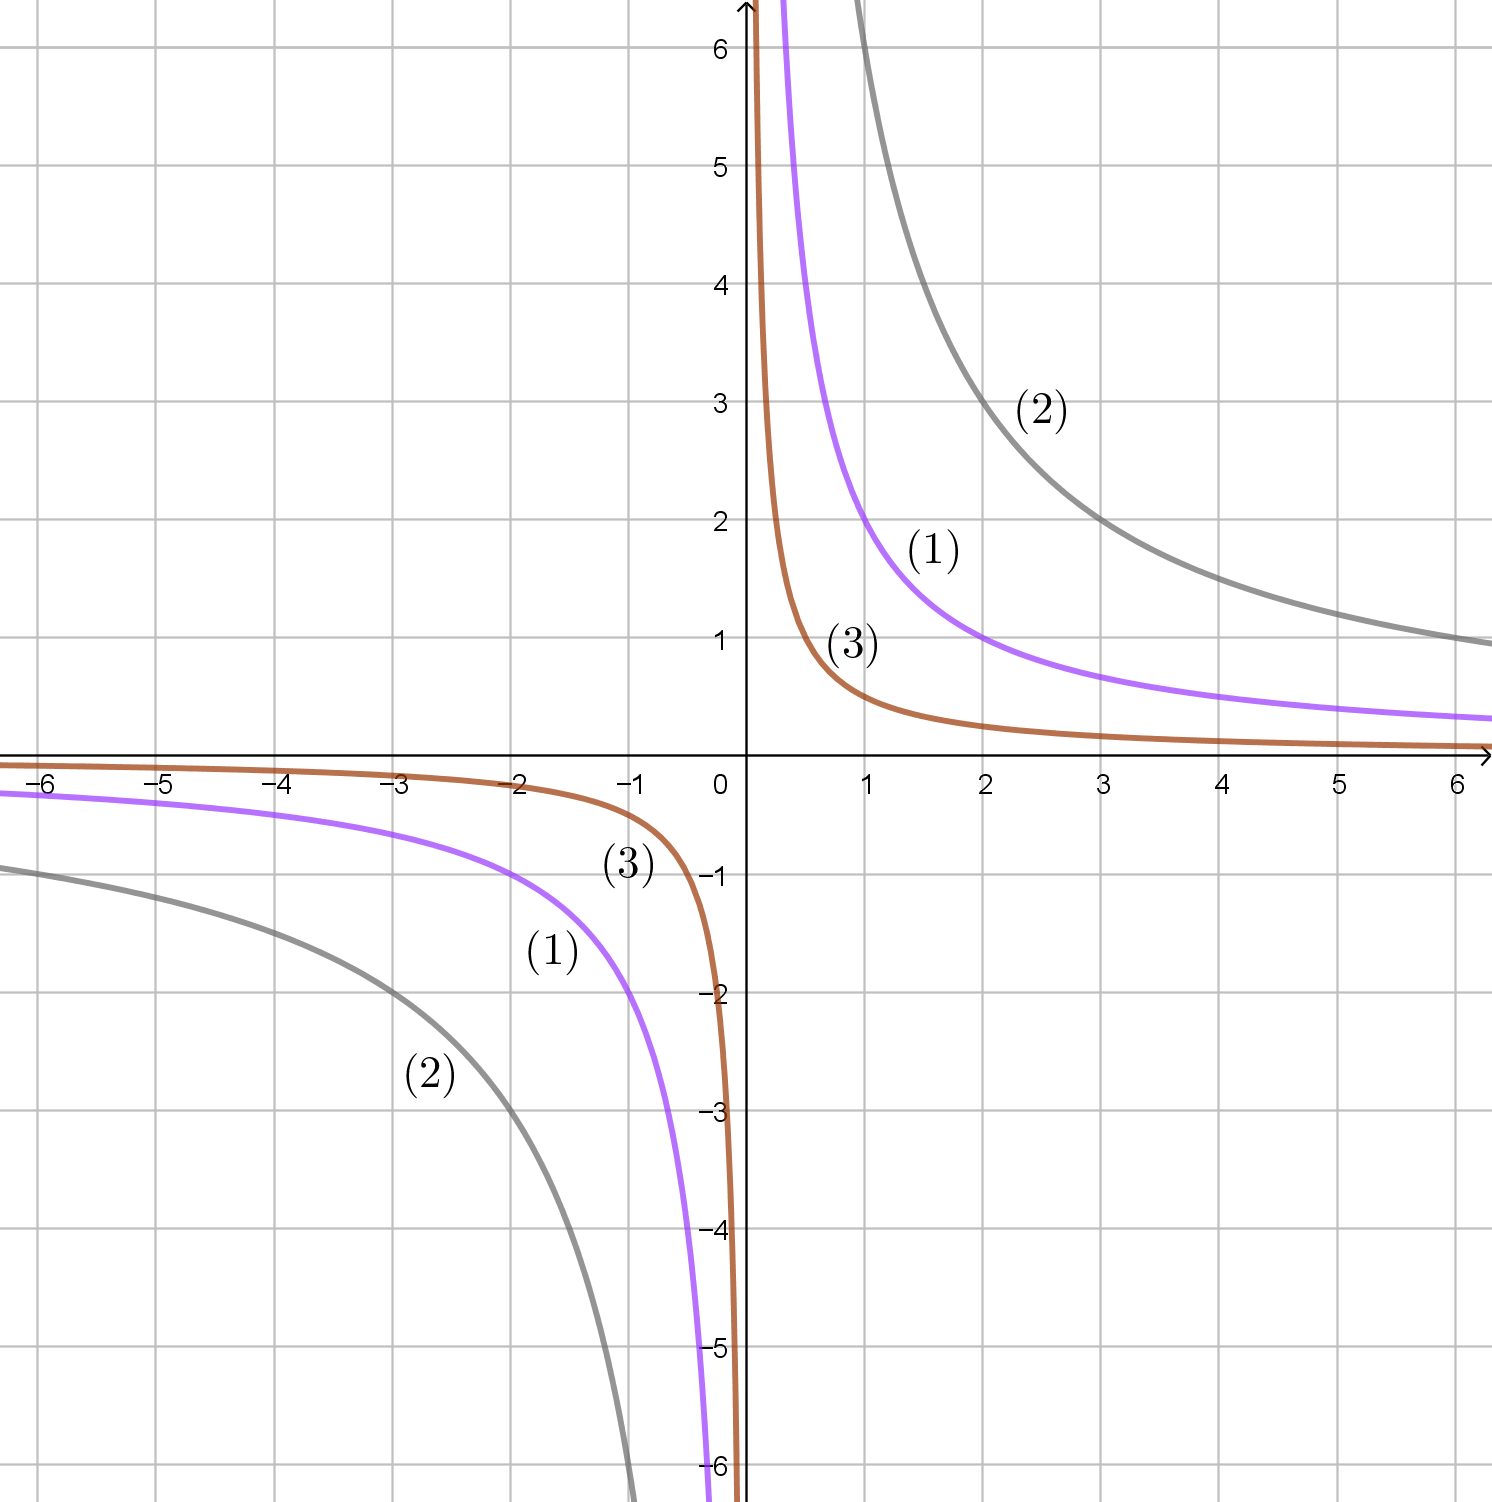
\includegraphics[width=0.8\columnwidth]{rational_2}
\end{center}

%
\an{rational5}
\begin{center}
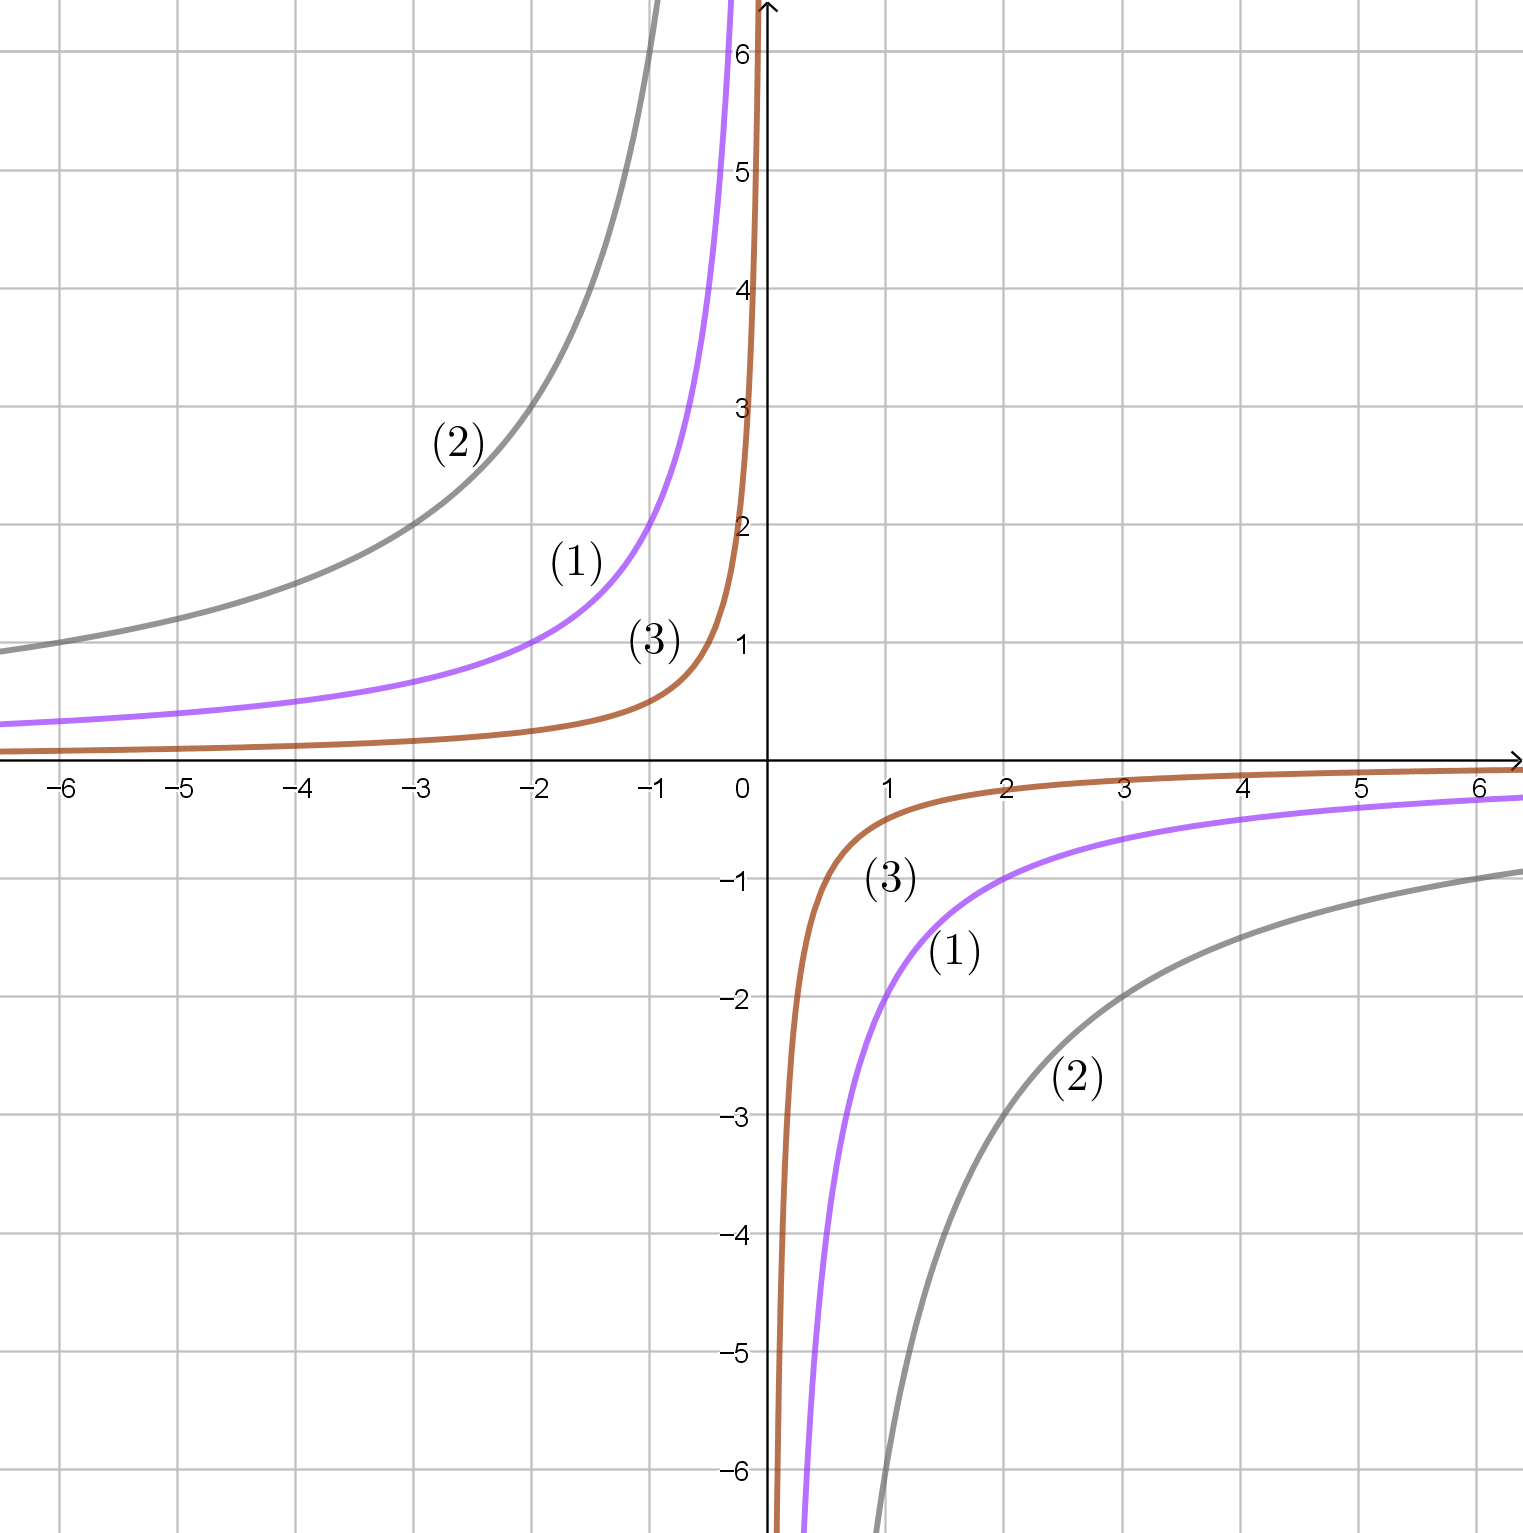
\includegraphics[width=0.8\columnwidth]{rational_5}
\end{center}

\columnbreak

%
\an{rational7}
\hspace{-.7em}
\(정의역=\{x\ba x\neq0\}\)\\
\(공역=\text{실수 전체의 집합}\)\\
\(치역=\{y\ba y\neq0\}\)

%
\an{rational9}
(1)
\begin{center}
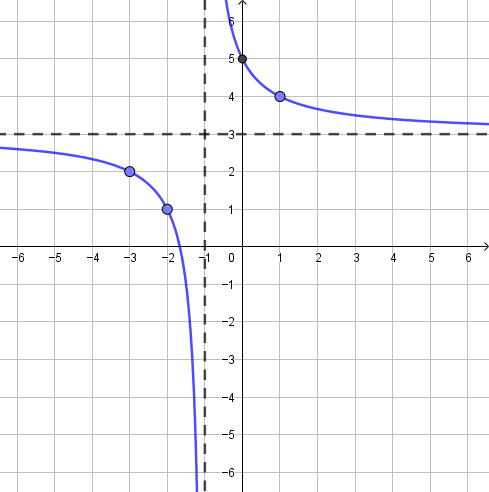
\includegraphics[width=0.8\columnwidth]{rational_9-1}
\end{center}
\parbox[t]{0.9\columnwidth}{점근선 : \(x=-1\), \(y=3\)\\\(x절편=-\frac53\),\qquad\(y절편=5\)}
\par\bigskip\noindent
(2)
\begin{center}
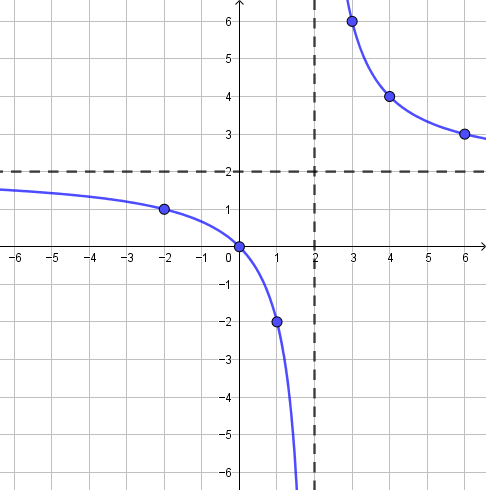
\includegraphics[width=0.8\columnwidth]{rational_9-2}
\end{center}
\parbox[t]{0.9\columnwidth}{점근선 : \(x=2\), \(y=2\)\\\(x절편=0\),\qquad\(y절편=0\)}
\par\columnbreak\noindent
(3)
\begin{center}
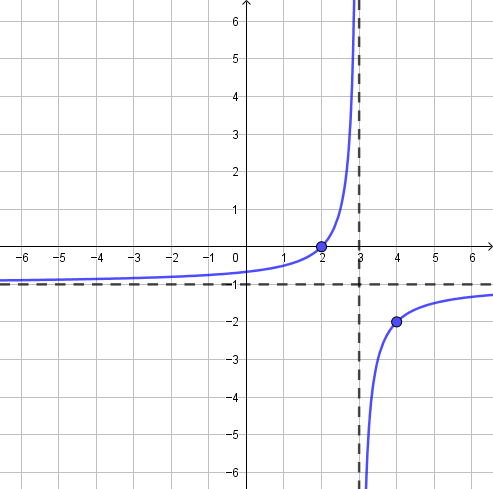
\includegraphics[width=0.8\columnwidth]{rational_9-3}
\end{center}
\parbox[t]{0.9\columnwidth}{점근선 : \(x=3\), \(y=-1\)\\\(x절편=2\),\qquad\(y절편=-\frac23\)}

%
\an{irrational4}
(1)
\begin{center}
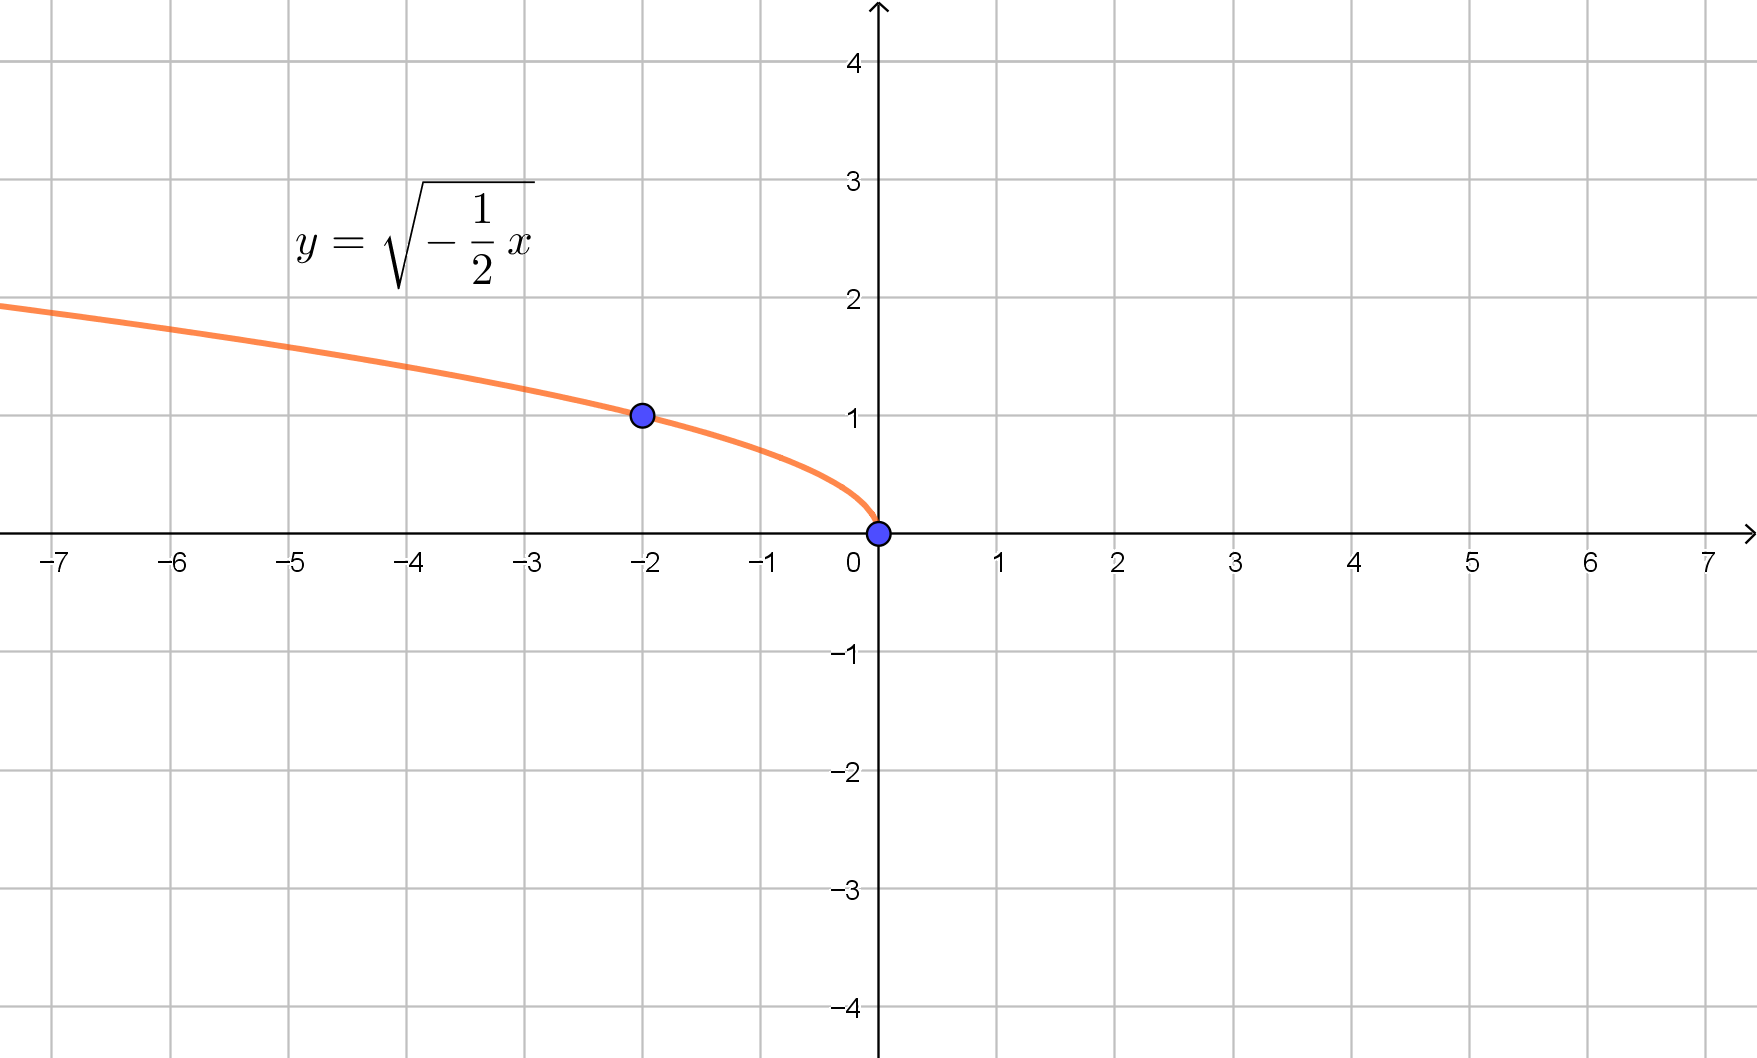
\includegraphics[width=0.99\columnwidth]{irrational_4-1}
\end{center}
\par\bigskip\noindent
(2)
\begin{center}
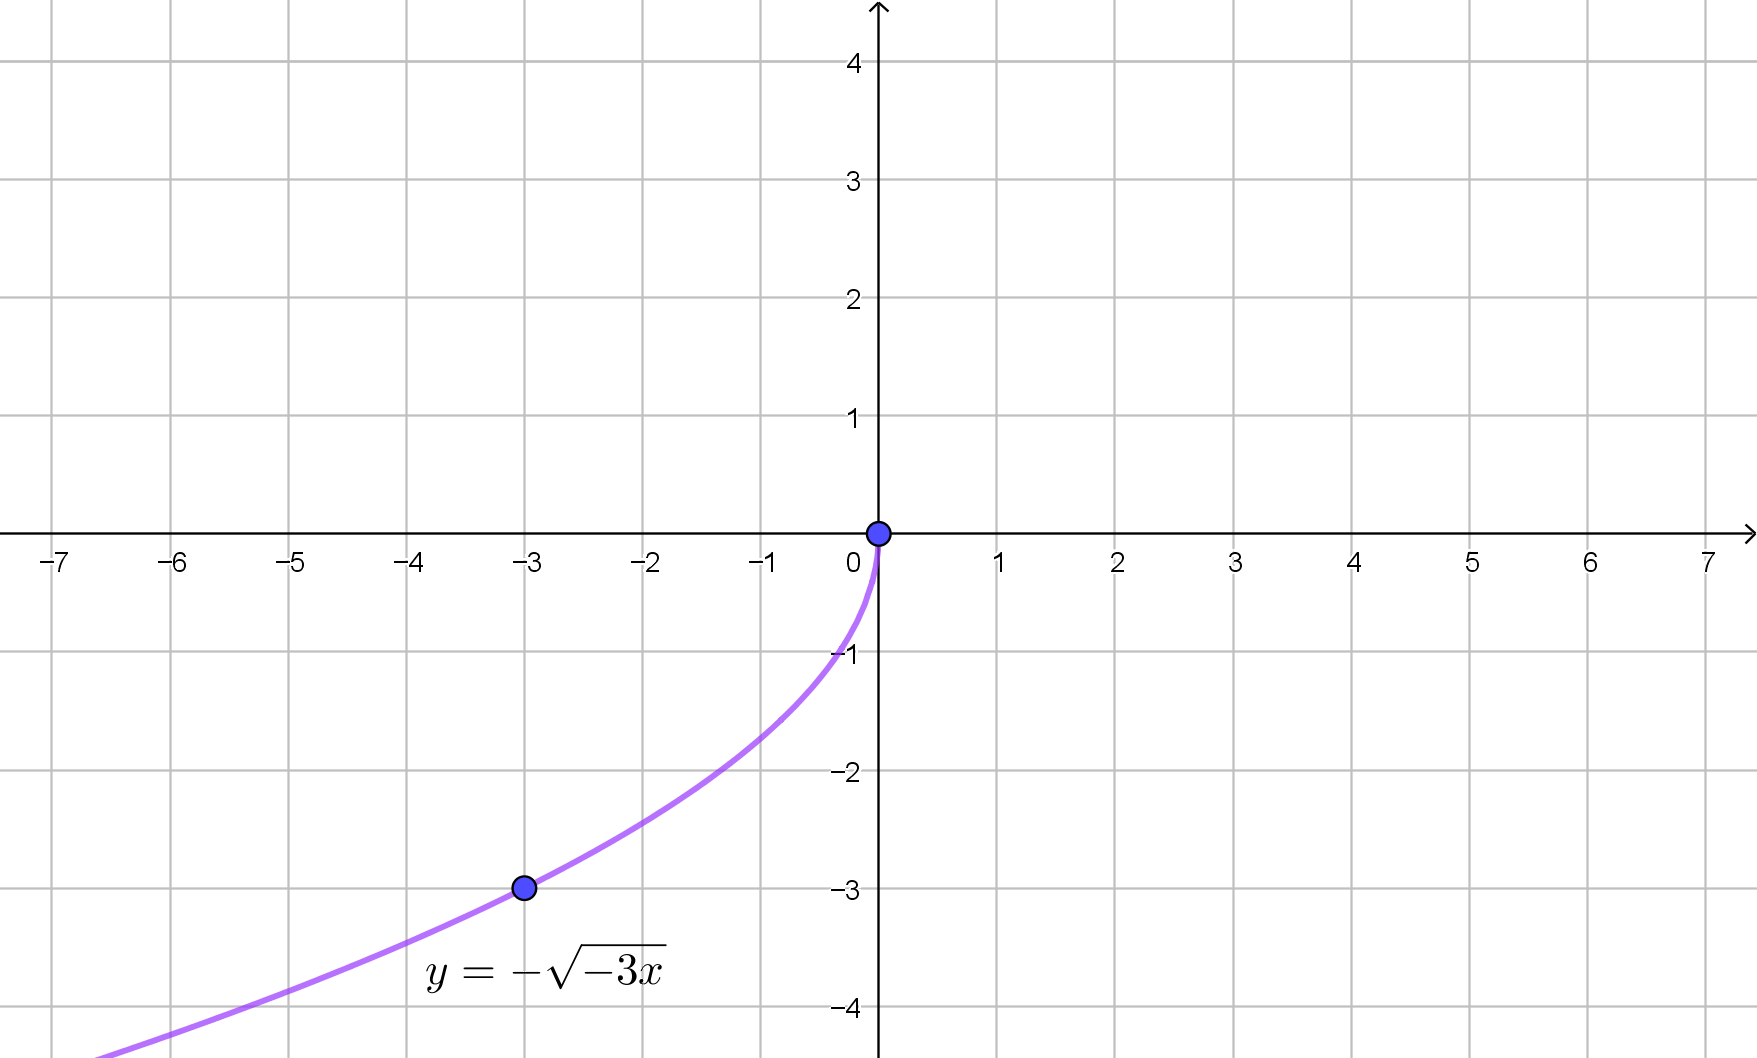
\includegraphics[width=0.99\columnwidth]{irrational_4-2}
\end{center}

\vfill\null\columnbreak

%
\an{irrational5}

\begin{center}
\scriptsize
\begin{tabu}to.99\columnwidth{X[1.2,$]|X[c,$]|@{}X[c,$]}
				&정의역		&치역\\\hline
y=\sqrt{-\frac12x}	&\{x\ba x\le0\}	&\{y\ba y\ge0\}\\
y=-\sqrt{-3x}		&\{x\ba x\le0\}	&\{y\ba y\le0\}
\end{tabu}
\end{center}

%
\an{irrational7}
(1)
\begin{center}
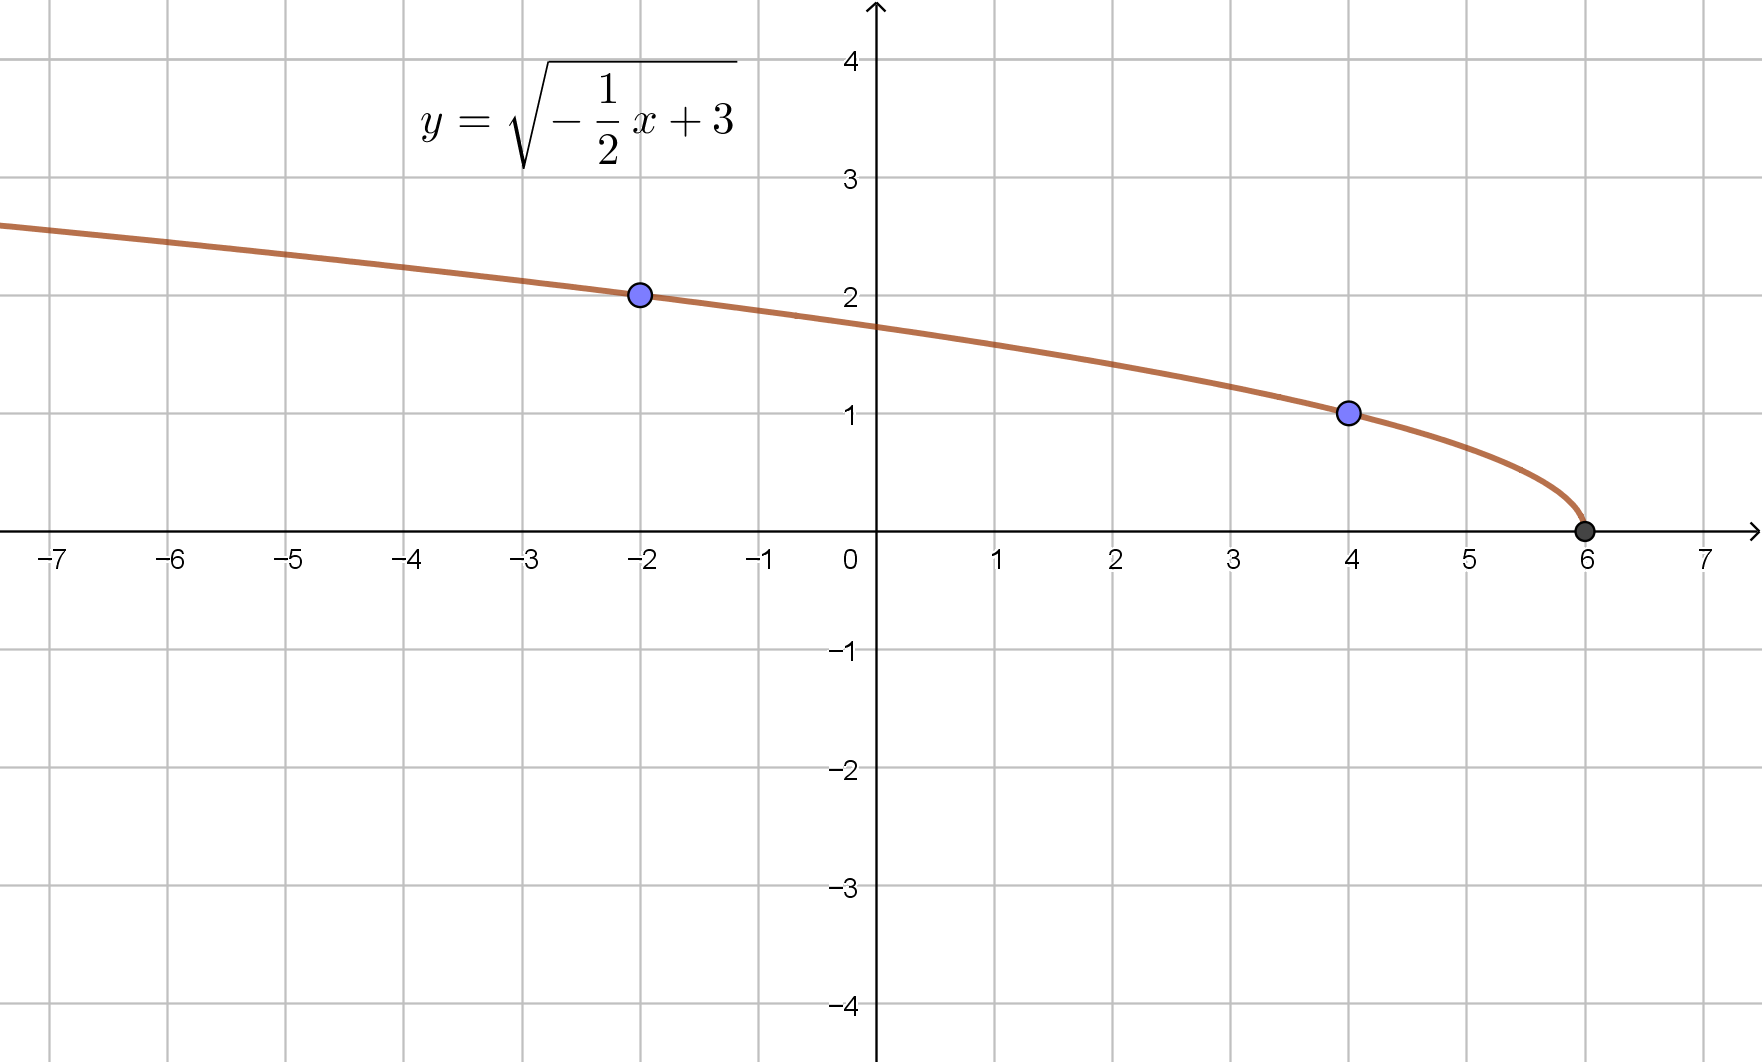
\includegraphics[width=0.99\columnwidth]{irrational_7-1}
\end{center}
\(x절편=6\),\qquad\(y절편=\sqrt3\)
\par\bigskip\noindent
(2)
\begin{center}
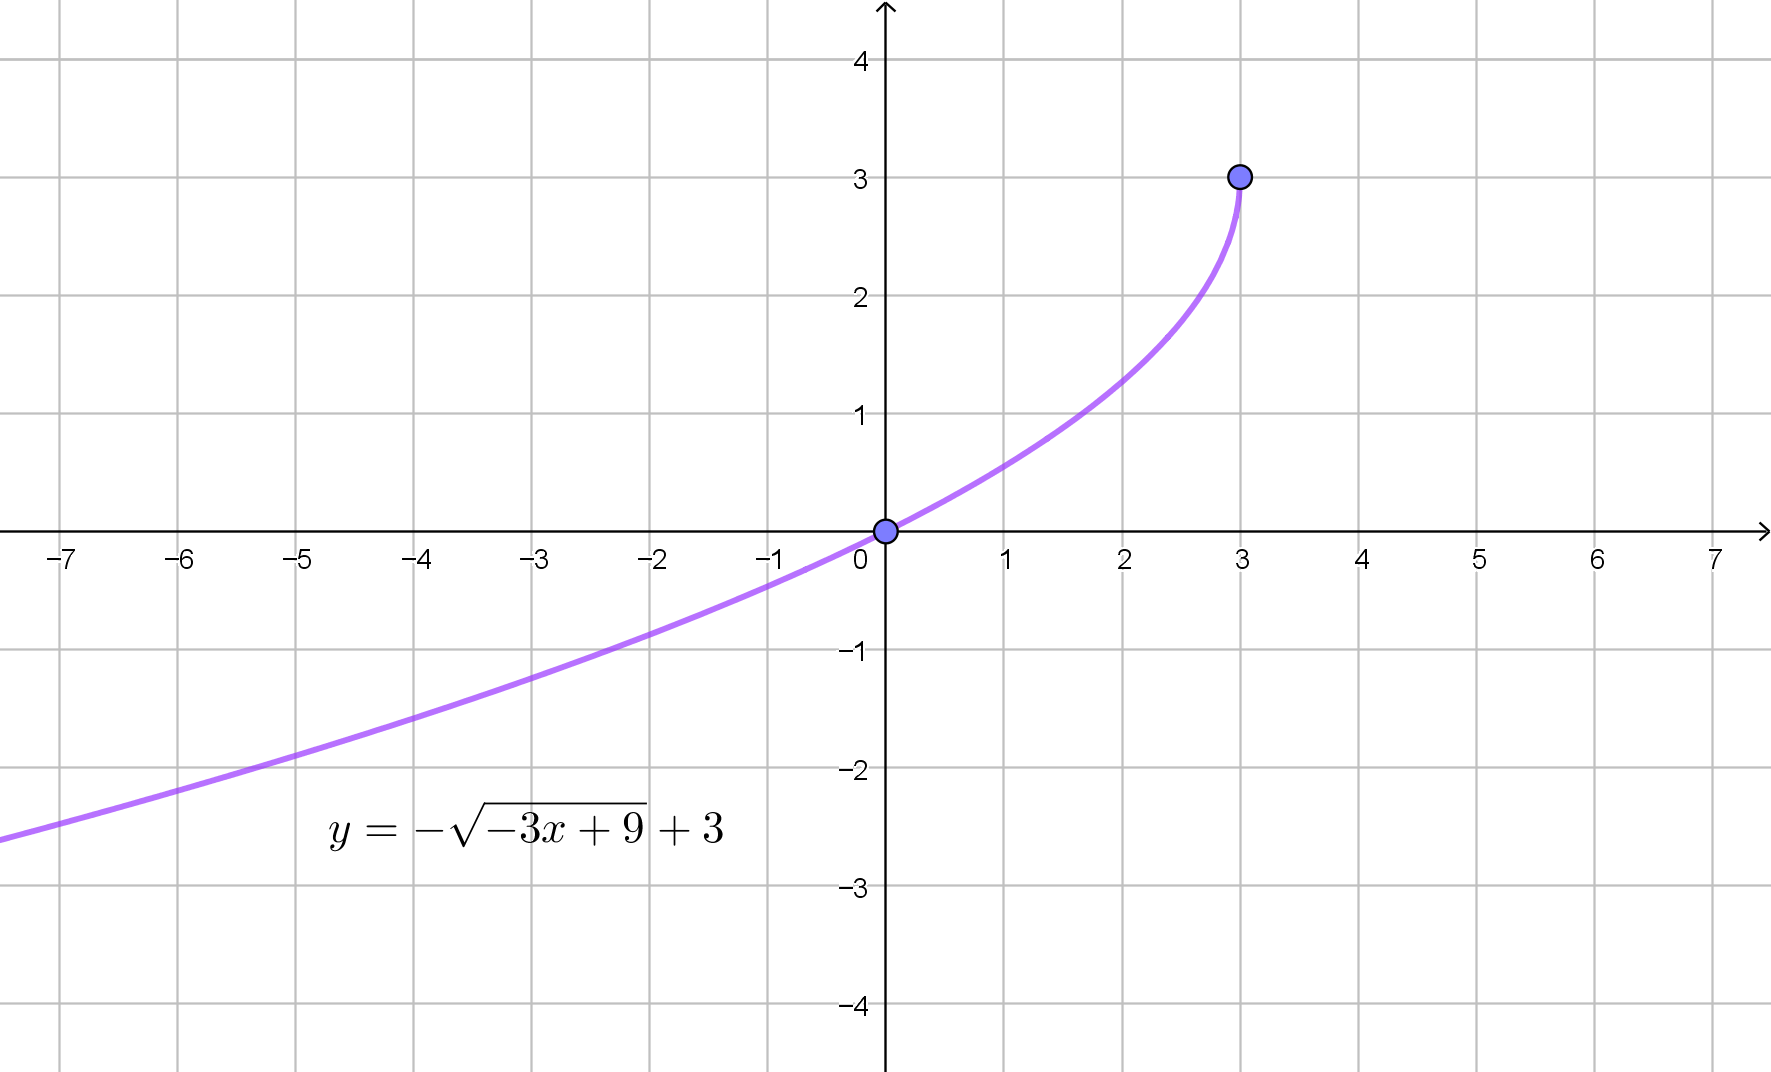
\includegraphics[width=0.99\columnwidth]{irrational_7-2}
\end{center}
\(x절편=0\),\qquad\(y절편=0\)
\end{multicols*}


%%
\section*{요약}
\addcontentsline{toc}{chapter}{\protect\numberline{*}요약}
\begin{enumerate}[label=\arabic*.,itemsep=15pt]
\item
유리함수 \(y=\frac1x\)의 그래프
\begin{center}
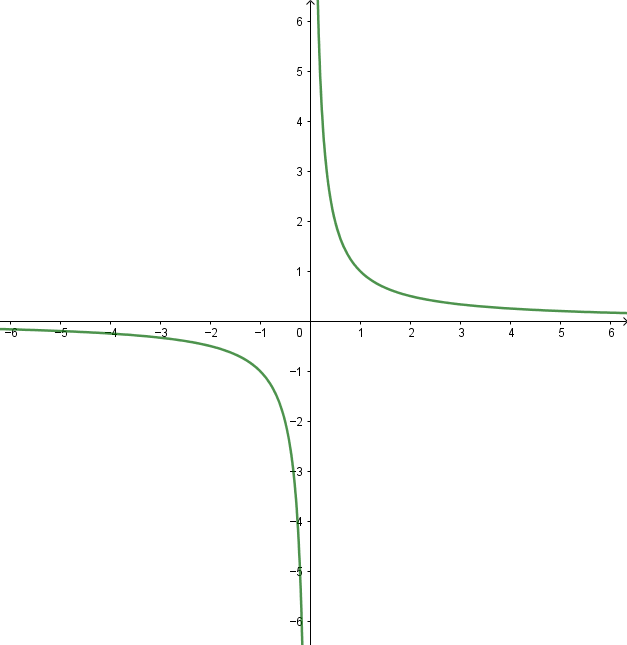
\includegraphics[width=0.6\textwidth]{summary_1-1}
\end{center}
\item
무리함수 \(y=\sqrt x\)의 그래프
\begin{center}
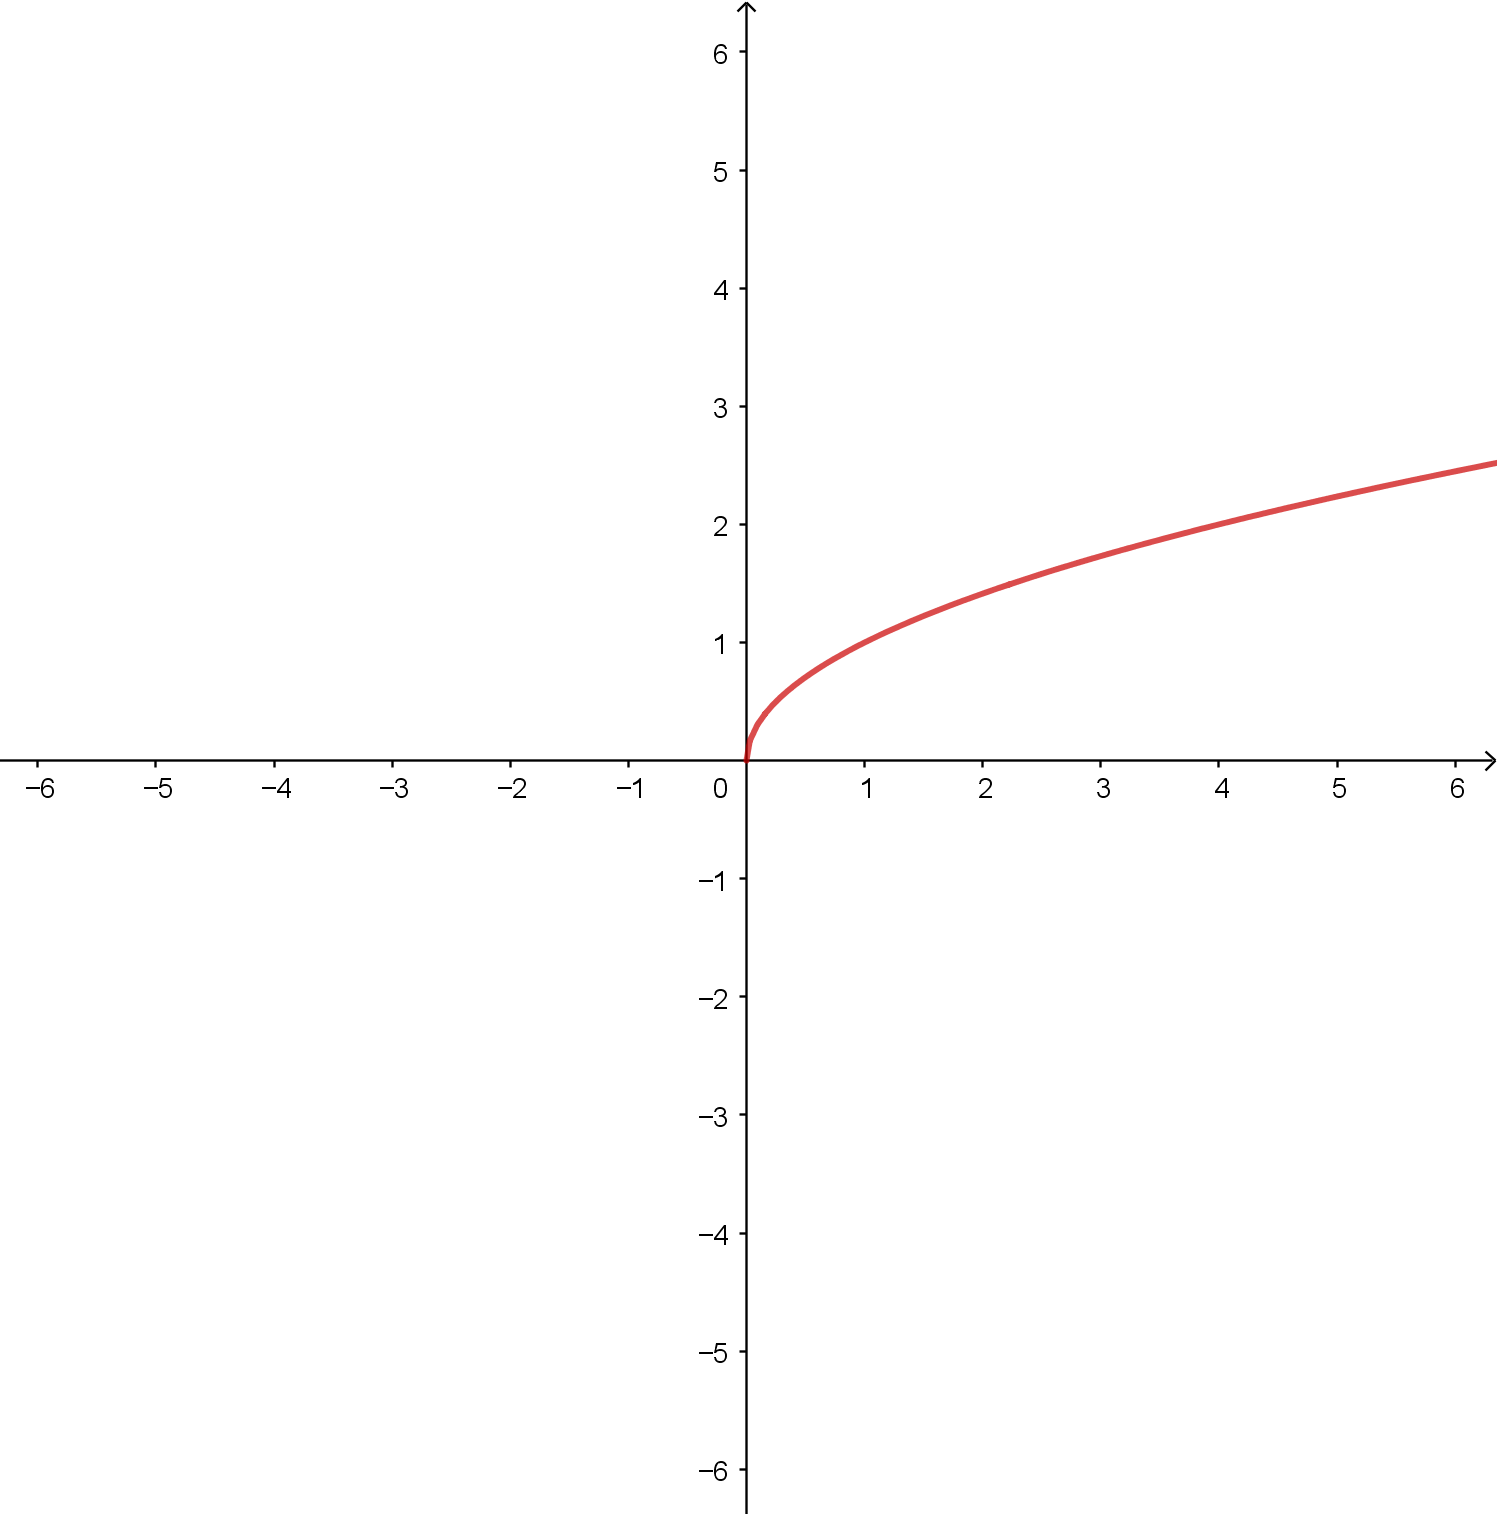
\includegraphics[width=0.6\textwidth]{summary_1-2}
\end{center}
\end{enumerate}

\end{document}